\documentclass[9pt, aspectratio=169]{beamer}

%! TEX root = ./root.tex
\let\Big\Huge
% \usetheme[width=15mm]{Berkeley}
\usetheme[width=15mm]{Hannover}
% \usecolortheme{seagull}
% \usecolortheme{sidebartab}
\usecolortheme{rose}
\usecolortheme{dolphin}

\usepackage[utf8]{inputenc}
\usepackage{%
	amsmath,
	amsfonts,
	amssymb,
	graphicx,
	xcolor,
	bookmark,
	subcaption,
	tikz,
	pgfplots,
	setspace,
	braket,
	booktabs,
	cleveref,
	qrcode
}
\usepackage[version = 4]{mhchem}
\usepackage[locale = DE, separate-uncertainty = true]{siunitx}
\usepackage[
	autocite=footnote,
	style=verbose,
	sorting=none,
	language=american,
	url=false,
	doi=false,
	isbn=false,
	eprint=false
]{biblatex}
\addbibresource{library.bib}
\usepgfplotslibrary{ternary}
\usetikzlibrary{%
	patterns,
	arrows.meta,
	shapes,
	trees,
	positioning,
	decorations.pathmorphing
}
\tikzstyle{every picture}+=[remember picture]
\linespread{1.1}

\definecolor{UFABC}{RGB}{0,90,60}

\setbeamertemplate{caption}[numbered]
\setbeamerfont{caption}{size=\footnotesize}
\setbeamerfont{footnote}{size=\tiny}
\setbeamercolor{structure}{fg=UFABC}

% \makeatletter
% \setbeamertemplate{sidebar \beamer@sidebarside}
% {%
% 	\beamer@tempdim=\beamer@sidebarwidth%
% 	% \advance\beamer@tempdim by -6pt%
% 	\vskip4em%
% 	\insertverticalnavigation{\beamer@sidebarwidth}%
% 	\vfill%
% 	\ifx\beamer@sidebarside\beamer@lefttext%
% 	\else%
% %		\usebeamercolor{normal text}%
% %		\usebeamercolor[]{}%
% 		\llap{\usebeamertemplate***{navigation symbols}\hskip5mm}%
% 		\vskip2pt%
% 	\fi%
% }%

% \setbeamertemplate{section in sidebar}%{sidebar theme}
% {%
% 	\vbox{%
% 		\vskip1ex%
% 		\beamer@sidebarformat{9pt}{section in sidebar}{\insertsectionhead}%
% 	}%
% }
% \setbeamertemplate{section in sidebar shaded}%{sidebar theme}
% {%
% 	\vbox{%
% 		\vskip1ex%
% 		\beamer@sidebarformat{9pt}{section in sidebar shaded}{\insertsectionhead}%
% 	}%
% }
% \makeatother

\AtBeginSection[]{%
	\begin{frame}
		\vfill
		\centering
		\usebeamerfont{title}\usebeamercolor[fg]{title}\insertsectionhead\par%
		\vfill
	\end{frame}
}

\AtBeginSubsection[]{%
	\begin{frame}
		\vfill
		\centering
		\usebeamerfont{title}\usebeamercolor[fg]{title}\insertsubsectionhead\par%
		\vfill
	\end{frame}
}

\setbeamertemplate{navigation symbols}{}%remove navigation symbols

\setbeamertemplate{frametitle}{%
	\vspace{4mm}%
	\usebeamerfont{title}%
	\insertframetitle%
	\hfill%
	\footnotesize%
	\insertframenumber/\inserttotalframenumber%
	\par%
	\nointerlineskip%
	\vspace{1mm}
	\hrulefill%
}

\newcommand\crule[3][black]{\textcolor{#1}{\rule{#2}{#3}}}
\renewcommand{\figurename}{Fig.}
\renewcommand{\tablename}{Tab.}

% Use shortjournal instead of journal from library.bib
\renewbibmacro*{journal}{%
  \iffieldundef{shortjournal}
    {%
      \iffieldundef{journaltitle}
        {}
        {%
          \printtext[journaltitle]
            {%
              \printfield[titlecase]{journaltitle}%
              \setunit{\subtitlepunct}%
              \printfield[titlecase]{journalsubtitle}%
             }%
         }%
    }
    {\printtext[journaltitle]{\printfield[titlecase]{shortjournal}}}%
}


\author[]{Alexandre O. Kraus, Jeverson T. Arantes}
\title[]{\bfseries \texorpdfstring{\ce{NaNbO3}}{NaNbO3} Vacancies Defects And Thin-film Biaxial Strain Effect}
\subtitle{A First-Principles Approach}
\date{Junho de 2021}
\institute{Defesa de Dissertação para o Programa de Pós-Graduação em Nanociências e Materiais Avançados}
\titlegraphic{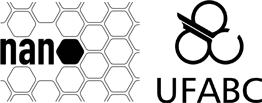
\includegraphics[height=40px]{../floats/agradecimentos/logo_nano_footer2.png}\hfill
\includegraphics[height=40px]{../floats/agradecimentos/logo-original-preta.pdf}}

\begin{document}

\tikzstyle{every picture}+=[remember picture]

% By default all math in TikZ nodes are set in inline mode. Change this to
% displaystyle so that we don't get small fractions.
\everymath{\displaystyle}

\tikzstyle{arrow} = [draw, -{Latex[width=0.5em]}]
\newcommand{\tikzmark}[1]{\tikz[baseline,remember picture] \coordinate (#1) {};}% TikZ aponta setas para onde o \titkzset está

\tikzset{%
    square arrow/.style={%
       to path={-- ++(-10,-.25) -| (\tikztotarget)}
  }
}

\frame{\titlepage}

%! TEX root = ../root/root.tex
\section{Introdução}

\begin{frame}[allowframebreaks]{Fotocatálise Da Água}
	\begin{columns}
		\begin{column}{.5\textwidth}
			\begin{figure}[t]
				\centering
				\def\svgwidth{\linewidth}
				\input{../floats/watersplitting.pdf_tex}
				\caption{Um semicondutor precisa ter limites be banda bem alinhados com os potenciais de oxirredução da água, além de uma banda proibida que permita absorção de luz visível/UV próximo.}
			\end{figure}
		\end{column}
		\begin{column}{.5\textwidth}
			\begin{block}{Produção de \ce{H2(g)}}
				\begin{itemize}
					\item \ce{H2(g)}: Alta densidade energética, queima limpa e renovável;
					\item Pode ser produzido por quebra da molécula de água catalisada por semicondutores.
				\end{itemize}
			\end{block}
			\begin{block}{Semicondutores Ideais}
				\begin{itemize}
					\item Alinhamento dos limites da banda proibida com os potenciais de oxirredução $+$ absorção de luz visível $+$ boa condutividade $+$ sítios ativos abundantes $+$ durabilidade.
				\end{itemize}
			\end{block}
		\end{column}
	\end{columns}\framebreak
	\begin{block}{Semicondutores Reais}
		\begin{itemize}
			\item Associação à cocatalizadores, células em camadas (\textit{tandem}) $\to$ perdas de eficiência e aumento do custo produtivo;
			\item \alert{\ce{NaTaO3} e \ce{NaNbO3} são vantajosos por não precisarem de cocatalizador!}
			\begin{itemize}
				\item Porém absorvem luz no UV $\to$ atividade fotocatalítica menor que semicondutores alternativos.
			\end{itemize}
		\end{itemize}
	\end{block}
	\begin{block}{Engenharia De Bandas: Controle De Defeitos}
		\begin{itemize}
			\item Defeitos com níveis rasos, pontuais ou de superfície $\to$ aumento da condutividade, redução do tamanho de banda proibida;
			\item Vacâncias: neutras, carregadas, concentração depende das condições de síntese;
			\item Superfícies: orientação, filme fino nanométrico ou não, tensão biaxial.
		\end{itemize}
	\end{block}
\end{frame}
\begin{frame}{Objetivos}
	\begin{block}{Dos Sistemas}
		\begin{itemize}
			\item Vacâncias isoladas de \ce{Na} e \ce{O}, neutras e carregadas.
			\item Filme finos de \ce{NaNbO3} e \ce{NaTaO3} ortorrômbicos, orientados em $[100]$, terminados em \ce{NaBO} (\ce{B} $=$ \ce{Nb, Ta});
			\item Tensão biaxial nos filmes finos.
		\end{itemize}
	\end{block}
	\begin{block}{A Entender}
		\begin{itemize}
			\item Como alteram a estrutura eletrônica do cristal volumoso? Podem beneficiar a fotocatálise?
			\item Como a tensão biaxial modula a estrutura de bandas da superfície orientada?
			\item Com quais condições químicas se controla a formação de vacâncias?
			\item O filme fino de \ce{NaTaO3} pode melhorar a fotocatálise. O filme fino de \ce{NaNbO3} tem mesma potencialidade?
		\end{itemize}
	\end{block}
\end{frame}

%! TEX root = ../root/root.tex 
\section{Metodologia e Métodos}

\begin{frame}{Métodos De Primeiros Princípios: DFT}
	\begin{figure}[t]
		\centering
		{\footnotesize%! TEX root = ../root/raiz.tex
\begin{tikzpicture}[node distance=3mm]
	\node [text width=12em, text centered] (step1) {$V_{\text{eff}} = V_{\text{ext}} + V_H[n] + V_{XC}[n]$};
	\node [below=of step1, text width=20em, text centered] (step2) {Resolver $(\hat{T} + V_{\text{eff}})\ket{\psi_i(\mathbf{r})} = \varepsilon_i \ket{\psi_i(\mathbf{r})}$ para $\varepsilon_i$};
	\node [below=of step2, text width=9em, text centered] (conv) {$\varepsilon_i - \varepsilon_{i-1} < \varepsilon_{\text{conv}}$?};
	\node [left=of conv, text width=10em] (newden) {$n_i(\mathbf{r}) = \braket{\psi_i(\mathbf{r}) | \hat{n} | \psi_i(\mathbf{r})}$};
	\node [right=of conv, text width=6em] (final) {Fim};
%%%%%%%%%%%%%%%%%%%%%%%%%%%%%%%%%%%%%%%%%%%%%%%%%%%%%%%%%%%%%%%%%%%%%%%%%%%%%%%
	\draw [arrow] (step1) -- (step2);
	\draw [arrow] (step2) -- (conv);
	\draw [arrow] (conv) -- node [anchor=west, xshift=-1.1em, yshift=1em] {não} (newden);
	\draw [arrow] (newden) |- (step1.west);
	\draw [arrow] (conv.east) -- node [anchor=east, xshift=1.1em, yshift=1em] {sim} (final.west);
\end{tikzpicture}
}
		\caption{Esquema autoconsistente da DFT para a obtenção do $\psi_0$.\label{fig:flowdft}}
	\end{figure}
	\begin{columns}
		\begin{column}{.175\textwidth}
			
\includegraphics[height=50px]{../floats/logo_vasp.png}
		\end{column}
		\begin{column}{.825\textwidth}\fontsize{7}{7}
			\begin{itemize}
				\item \textit{Vienna Ab initio Simulation Package} (VASP)\footnote[frame]{\cite{kresse_efficient_1996,kresse_ultrasoft_1999}} usado com GGA-PBE;
				\item Contagem de elétrons nas vizinhanças de cada átomo com a abordagem \emph{Atoms In Molecules}\footnote[frame]{\cite{bader_quantum_1981}};
				\item Parâmetros de rede do cristal volumoso obtidos por minimização da energia total\footnote[frame]{\cite{george_effect_2018,hu_influence_2007}}:
				\begin{itemize}\footnotesize
					\item[\ce{NaNbO3}.] $a = 5.62$ ($+1.1\%$), $b = 7.90$ ($+0.9\%$) e $c = \SI{5.55}{\angstrom}$ ($+1.4\%$);
					\item[\ce{NaTaO3}.] $a = 5.62$ ($+2.0\%$), $b = 7.86$ ($+0.9\%$) e $c = \SI{5.58}{\angstrom}$ ($+1.1\%$).
				\end{itemize}
			\end{itemize}
		\end{column}
	\end{columns}
\end{frame}
\begin{frame}{Propriedades Cristalinas}
	\begin{columns}
		\begin{column}{.4\textwidth}
			\begin{figure}[t]
				\centering
				\input{../floats/bond_angles/bond_angles.pdf_tex}
				\caption{Ângulos de ligação \ce{Nb-O-Nb} $\alpha$ (direção $[\overline{1}01]$), $\beta$ (direção $[101]$), $\gamma$ (direção $[010]$).\label{fig:angles}}
			\end{figure}
		\end{column}
		\begin{column}{.5\textwidth}{\small
			\begin{itemize}
				\item Distância de ligação \ce{Nb-O} média ($\overline{d_{\ce{Nb-O}}}$) e comparação com o do cristal volumoso em estado fundamental;
				\item Ângulos entre octaedros em referência aos seus eixos, nas direções cristalinas: $[\overline{1}01]$ ($\alpha$), $[101]$ ($\beta$) e $[010]$ ($\gamma$);
				\item Distorção dos octaedros avaliada com o índice de Baur\footnote[frame]{\cite{baur_geometry_1974}}:
				\begin{equation}
					\Delta_d = \frac{1}{6} \sum^{6}_{i=1} \frac{|d_{\ce{Nb-O}\, i} - \overline{d_{\ce{Nb-O}}}|}{\overline{d_{\ce{Nb-O}}}};
				\end{equation}
				\item Filme finos: superfícies formam tetraedros \ce{NbO4}. Repulsão dos orbitais $p-d$ depende do ângulo de ligação \ce{O-Nb-O}. O índice de planaridade $P_L$ descreve quâo próximo está do ideal:
				\begin{equation}
					P_L = \frac{\theta_{\ce{O-Nb-O}}}{\SI{180}{\degree}};
				\end{equation}
			\end{itemize}}
		\end{column}
	\end{columns}
\end{frame}
\begin{frame}{Estimativa Da Energia De Formação De Vacância}
	\begin{itemize}{\small%
		\item A energia de formação $\Delta E_f$ para vacâncias v$_{\ce{X}}^{q} = \text{v}_{\ce{O}}^{0}, \text{v}_{\ce{O}}^{2+}, \text{v}_{\ce{Na}}^{0}, \text{v}_{\ce{Na}}^{1-}$:
		\begin{equation}
			\Delta E_f (\text{v}_{\ce{X}}^{q}; L) =
			\tikz[baseline] {\node[anchor=base, fill=red!50] (part1) {$\!E_T (\text{v}_{\ce{X}}^{q}; L)\!$};} -
			\tikz[baseline] {\node[anchor=base, fill=green!40] (part2) {$\!E_T (\text{perfeito}; L)\!$};} -
			\tikz[baseline] {\node[anchor=base, fill=blue!50] (part3) {$\!n_{\ce{X}} \mu_{\ce{X}}\!$};} +
			\tikz[baseline] {\node[anchor=base, fill=violet!50] (part4) {$\!q \varepsilon_F\!$};} +
			\tikz[baseline] {\node[anchor=base, fill=black!40] (part5) {$\!E_c$};}.
		\end{equation}
		\begin{itemize}
			\footnotesize
			\item\tikz{\node [fill=red!50] (description1) {Energia total da supercélula com v${}_{\ce{X}}^{q}$;};}
			\item\tikz{\node [fill=green!40] (description2) {Energia total do cristal volumoso sem defeitos;};}
			\item\tikz{\node [fill=blue!50] (description3) {Troca com reservatório de \ce{X};};}
			\item\tikz{\node [fill=violet!50] (description4) {Troca com reservatório de e${}^{-}$;};}
			\item\tikz{\node [fill=black!40] (description5) {Correção de preenchimento de banda.};}
		\end{itemize}
		\item Interações vacância-imagens $\to$ imprecisão na energia de formação $\propto L = V^{{}^{1}\!/{}_{3}}$;
		\item Extrapolação $L\to\infty$ (limite diluído) modelada com\footnote[frame]{\cite{castleton_managing_2006}}:
		\begin{equation}
			\Delta E_f (\text{v}_{\ce{X}}^{q}; L) = \Delta E_f (\text{v}_{\ce{X}}^{q}; L\to\infty) + a_1 L^{-1} + a_3 L^{-3}.
		\end{equation}
		\begin{itemize}
			\item Supercélulas repetem a célula convencional nos eixos cartesianos: $1\!\times\!1\!\times\!1$, $2\!\times\!2\!\times\!2$ e $3\!\times\!3\!\times\!3$;
			\item Parâmetros $\Delta E_f (\text{v}_{\ce{X}}^{q}; L\to\infty)$, $a_1$ e $a_3$ determinados pelo método dos mínimos quadrados.
		\end{itemize}
		}
	\end{itemize}
\end{frame}
\begin{frame}{Estimativa Da Energia De Formação De Vacância: Potencial Químico}
	\begin{columns}
		\begin{column}{.45\textwidth}
			\begin{figure}[t]
				\centering
				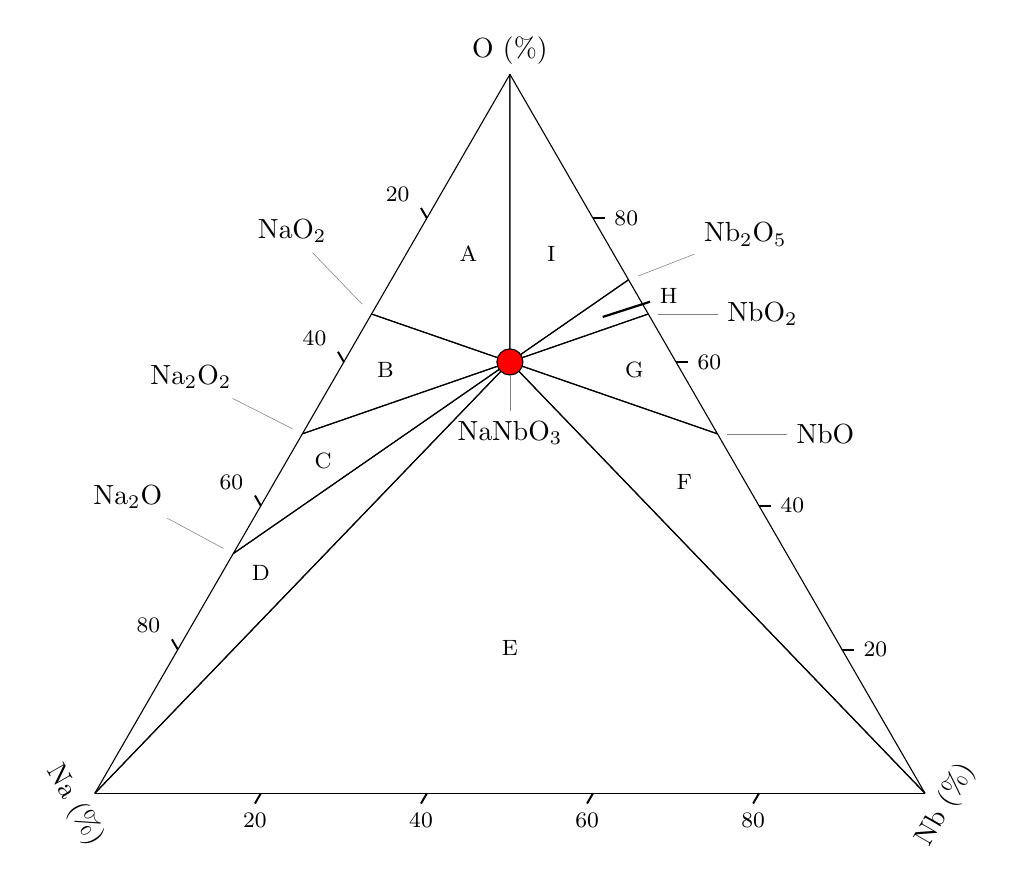
\begin{tikzpicture}
        \begin{ternaryaxis}[
        width=\textwidth,
        xlabel=O ($\%$),
        xlabel style={%
                at={(axis cs:1,0,0)},
                anchor=south
        },
        xtick={0.2,0.4,0.6,0.8},
        xticklabels={$20$,$40$,$60$,$80$},
        xticklabel style={font=\footnotesize},
        xtick style={line width=0.25mm, color=black},
        ylabel=Na ($\%$),
        ylabel style={%
                at={(axis cs:0,1,0)},
                anchor=north,
                rotate=-60
        },
        ytick={0.2,0.4,0.6,0.8},
        yticklabels={$20$,$40$,$60$,$80$},
        yticklabel style={font=\footnotesize},
        ytick style={line width=0.25mm, color=black, font=\tiny},
        zlabel=Nb ($\%$),
        zlabel style={%
                at={(axis cs:0,0,1)},
                anchor=north,
                rotate=60
        },
        ztick={0.2,0.4,0.6,0.8},
        zticklabels={$20$,$40$,$60$,$80$},
        zticklabel style={font=\footnotesize},
        ztick style={line width=0.25mm, color=black, font=\tiny},
        clip=false,
        no markers,
        grid=none
        ]
                \addplot3 [color=black] table {%
                        O        Na       Nb 
                        1.0      0.0      0.0
                        0.6      0.2      0.2
                        0.666667 0.333333 0.0
                };
            
                \addplot3 [color=black] table {%
                        O        Na       Nb 
                        0.666667 0.333333 0.0
                        0.6      0.2      0.2
                        0.5      0.5      0.0
                };
            
                \addplot3 [color=black] table {%
                        O        Na       Nb 
                        0.5      0.5      0.0
                        0.6      0.2      0.2
                        0.333333 0.666667 0.0
                };
            
                \addplot3 [color=black] table {%
                        O        Na       Nb 
                        0.333333 0.666667 0.0
                        0.6      0.2      0.2
                        0.0      1.0      0.0
                };
            
                \addplot3 [color=black] table {%
                        O        Na       Nb 
                        0.0      1.0      0.0
                        0.6      0.2      0.2
                        0.0      0.0      1.0
                };
            
                \addplot3 [color=black] table {%
                        O        Na       Nb 
                        0.0      0.0      1.0
                        0.6      0.2      0.2
                        0.5      0.0      0.5
                };
            
                \addplot3 [color=black] table {%
                        O        Na       Nb      
                        0.5      0.0      0.5     
                        0.6      0.2      0.2     
                        0.666667 0.0      0.333333
                };
            
                \addplot3 [color=black] table {%
                        O        Na       Nb      
                        0.714286 0.0      0.285714
                        0.6      0.2      0.2     
                        0.666667 0.0      0.333333
                };
            
                \addplot3 [color=black] table {%
                        O        Na       Nb      
                        0.714286 0.0      0.285714
                        0.6      0.2      0.2     
                        1.0      0.0      0.0     
                };
            
                \node [circle, draw, fill=red, pin={[pin distance=3ex]270:\ce{NaNbO3}}] at (axis cs:0.6,0.2,0.2) {};
                \node [pin={[pin distance=5ex]120:\ce{NaO2}}] at (axis cs:0.666667, 0.333333, 0.0) {};
                \node [pin={[pin distance=5ex]150:\ce{Na2O2}}] at (axis cs:0.5, 0.5, 0.0) {};
                \node [pin={[pin distance=5ex]150:\ce{Na2O}}] at (axis cs:0.333333, 0.666667, 0.0) {};
                \node [pin={[pin distance=5ex]0:\ce{NbO}}] at (axis cs:0.5, 0.0, 0.5) {};
                \node [pin={[pin distance=5ex]0:\ce{NbO2}}] at (axis cs:0.666667, 0.0, 0.333333) {};
                \node [pin={[pin distance=5ex]20:\ce{Nb2O5}}] at (axis cs:0.714286, 0.0, 0.285714) {};
        
                \node [] at (cartesian cs:0.45, 0.65) {{\footnotesize A}};
                \node [] at (cartesian cs:0.35, 0.51) {{\footnotesize B}};
                \node [] at (cartesian cs:0.275, 0.4) {{\footnotesize C}};
                \node [] at (cartesian cs:0.2, 0.265) {{\footnotesize D}};
                \node [] at (cartesian cs:0.5, 0.175) {{\footnotesize E}};
                \node [] at (cartesian cs:0.71, 0.375) {{\footnotesize F}};
                \node [] at (cartesian cs:0.65, 0.51) {{\footnotesize G}};
                \node [pin={[pin distance=4ex, pin edge={black, thick}]7.5:{\footnotesize H}}] at (cartesian cs:0.6, 0.57) {};
                \node [] at (cartesian cs:0.55, 0.65) {{\footnotesize I}};
        \end{ternaryaxis}
\end{tikzpicture}
				\caption{Diagrama ternário do \ce{NaNbO3} mostrando as regiões onde se avaliou $\mu_{\ce{X}}$ de v$_{\ce{X}}^q$.\label{fig:ternarypd}}
			\end{figure}
		\end{column}
		\begin{column}{.55\textwidth}
			\begin{itemize}
				\item Equilíbrio químico com o \ce{NaNbO3}: $\mu^{0}_{\ce{NaNbO3}} = \mu_{\ce{Na}} + \mu_{\ce{Nb}} + 3 \mu_{\ce{O}}$;
				\item Condições de síntese mudam $\mu_{\ce{X}}$, variando dentro dos limites impostos pelos reagentes e.g. no equilíbrio I:
				\begin{equation*}
					\begin{cases}
						2 \mu_{\ce{O}} = \mu_{\ce{O2}}^{0};\\
						2 \mu_{\ce{Nb}} + 5 \mu_{\ce{O}} = \mu_{\ce{Nb2O5}}^{0};\\
						\mu_{\ce{Na}} + \mu_{\ce{Nb}} + 3 \mu_{\ce{O}} = \mu_{\ce{NaNbO3}}^{0}.
					\end{cases} \Rightarrow
				\end{equation*}
				\begin{equation}
					\begin{cases}
						\mu_{\ce{O}} = {}^{1}\!/{}_{2}\, \mu_{\ce{O2}}^{0};\\
						\mu_{\ce{Nb}} = {}^{1}\!/{}_{2}\, \mu_{\ce{Nb2O5}}^{0} + {}^{5}\!/{}_{4}\, \mu_{\ce{Nb2O5}}^{0};\\
						\mu_{\ce{Na}} = \mu_{\ce{NaNbO3}}^{0} - {}^{1}\!/{}_{2}\, \mu_{\ce{Nb2O5}}^{0} - {}^{1}\!/{}_{4}\, \mu_{\ce{O2}}^{0}.
					\end{cases}
				\end{equation}
			\end{itemize}
		\end{column}
	\end{columns}
\end{frame}
\begin{frame}{Estudo Dos Filmes Finos}
	\begin{columns}
		\begin{column}{.5\textwidth}
			\begin{figure}[t]
				\centering
				\input{../floats/slabs/slabs.pdf_tex}
				\caption{Filme fino de \ce{NaNbO3}. Filme de \ce{NaTaO3} construído de maneira análoga.\label{fig:slabs}}
			\end{figure}
		\end{column}
		\begin{column}{.5\textwidth}
			\begin{itemize}
				\item Supercélula: célula convencional $\times 3$ em $[100]$ $+$ vácuo de \SI{15}{\angstrom};
				\begin{itemize}
					\item 9 camadas atômicas, 86 átomos.
				\end{itemize}
				\item Orientação da clivagem em $[100]$ e terminação \ce{NaNbO} $\to$ tetraedros \ce{NbO4};
				\item Remoção de duas ligações \ce{Nb-O} $\to$ carga formal $\to$ reconstrução de superfície;
				\item Estado fundamental descrito com \alert{$b$ e $c$ $1\%$ maiores que do cristal volumoso} $\to$ referência para tensão biaxial.
				\item Filme de \ce{NaTaO3} construído da mesma forma, estado fundamental com $b$ e $c$ idênticos ao do cristal volumoso. Uso em fotocatálise discutido em outro trabalho\footnote[frame]{\cite{kraus_modulation_2020}}.
			\end{itemize}
		\end{column}
	\end{columns}
	\begin{center}
		Figuras da dissertação no \href{https://github.com/o-aleoli/nma_dissertation_fig}{\color{blue}{repositório do GitHub}}.
	\end{center}
\end{frame}

%! TeX root = ../root/root.tex 
\section{Resultados}

\subsection{Vacâncias No Cristal Volumoso}
\begin{frame}[allowframebreaks]{Densidade de Estados Projetada -- Defeitos Neutros}
	\begin{figure}[t]
		\centering
		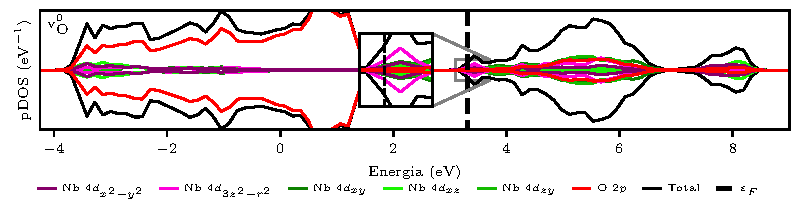
\includegraphics{../floats/pdos_vac/pdos_neutral_d_separated_333_vO.pdf}
		\caption{pDOS do v$_{\ce{O}}^0$ na supercélula $3\times3\times3$. Linha tracejada indica o nivel de Fermi ($\varepsilon_F$).\label{fig:pdosNeuVac_vO}}
	\end{figure}
	\begin{itemize}
		\item Átomo de \ce{O} removido $\to$ redução no nível energético de \ce{Nb} $4d_{3z^2-r^2}$ $+$ preenchimento parcial $\to$ \alert{níveis rasos doadores};
		\begin{itemize}
			\item \ce{O} apical removido $\to$ quebra da degenerescência $e_g$ $\to$ níveis \ce{Nb} $4d_{3z^2-r^2}$ abaixam ao remover a sobreposição de orbitais $p-d$;
			\item Nível de defeito \SI{27}{\milli\electronvolt} abaixo da condução $\to$ perto de ionizar com energia térmica ($300 k_B \approx \SI{26}{\milli\electronvolt}$);
			\item Pode haver \alert{aumento da densidade de elétrons} sem grande impacto à condutividade $\to$ melhora na reação de evolução de hidrogênio;
		\end{itemize}
	\end{itemize}\framebreak
	\begin{figure}[t]
		\centering
		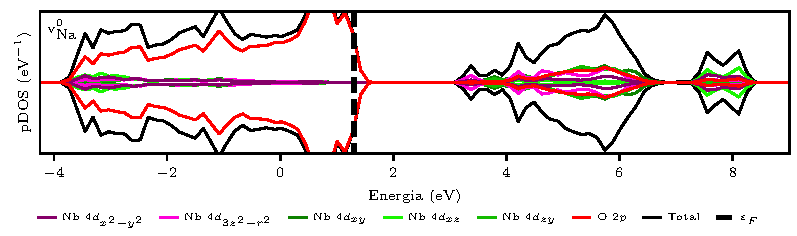
\includegraphics{../floats/pdos_vac/pdos_neutral_d_separated_333_vNa.pdf}
		\caption{pDOS do v$_{\ce{Na}}^0$ na supercélula $3\times3\times3$. Linha tracejada indica o nivel de Fermi ($\varepsilon_F$).\label{fig:pdosNeuVac_vNa}}
	\end{figure}
	\begin{itemize}
		\item Átomo de \ce{Na} removido $\to$ aumento do nível energético de \ce{O} $2p$ $+$ depleção parcial $\to$ \alert{níveis rasos aceitadores};
		\begin{itemize}
			\item Quebra de ligações \ce{Na-O} $\to$ orbitais \ce{O} $2p$ parcialmente preenchidos;
			\item Nível de defeito \SI{10}{\milli\electronvolt} acima da valência $\to$ ionização por energia térmica permitida;
			\item Pode haver \alert{aumento da densidade de lacunas} sem grande impacto na condutividade $\to$ melhora na reação de evolução de oxigênio;
		\end{itemize}
	\end{itemize}\framebreak
\end{frame}
\begin{frame}{Estrutura Cristalina}
	\begin{figure}[htb]
		\centering
		\input{../floats/geometry_vac/neighborhood_o0.pdf_tex}
		\caption{O arranjo atômico maios próximo ao defeito pontual antes (esquerda) e depois (direita) de formado. Após relaxação atômica, os \ce{O} (vermelho) equatoriais se aproximam do defeito enquanto os \ce{Nb} se afastam. Os ângulos \ce{Nb-O-Nb} dos \ce{O} equatoriais diminuem.}
	\end{figure}
	\begin{itemize}
		\item Vacância de \ce{O}: \ce{Nb} vizinhos se aproximam dos \ce{O} que formam o \ce{NbO5} compensando elétrons na valência do \ce{Nb};
		\item Vacância de \ce{Na}: preservação da disposição atômica anterior ao defeito pontual;
		\item Intensidade das ligações \ce{Nb-O} \textit{vs.} \ce{Na-O};
	\end{itemize}
\end{frame}
\begin{frame}[allowframebreaks]{Densidade De Estados Projetada -- Defeitos Com Carga}
	\begin{figure}[t]
		\centering
		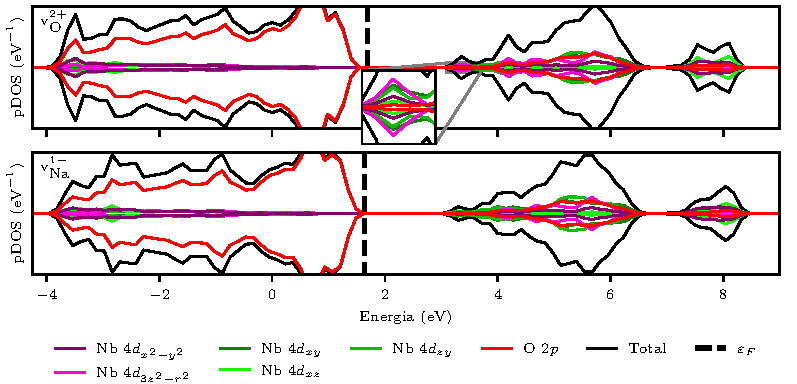
\includegraphics[scale=1]{../floats/pdos_vac/pdos_charged_d_separated_333.pdf}
		\caption{pDOS com v$_{\ce{O}}^{2+}$ e com v$_{\ce{Na}}^{1-}$ em supercélulas $3\times3\times3$. Linha tracejada indica o nivel de Fermi ($\varepsilon_F$).\label{fig:pdosChaVac}}
	\end{figure}\framebreak
	\begin{itemize}
		\item Ionização pouco altera a distância dos níveis energéticos de defeito pontial em relação aos limites de banda;
		\item Níveis de defeito do v${}_{\ce{O}}^{2+}$ esvaziados;
		\item Níveis de defeito do v${}_{\ce{Na}}^{1-}$ preenchidos;
		\item Tamanho da banda proibida: de \SI{1.91}{\electronvolt} foi para \SI{1.95}{\electronvolt} com v$_{\ce{O}}^{2+}$ e \SI{1.96}{\electronvolt} com v$_{\ce{Na}}^{1-}$;
		\begin{itemize}
			\item Níveis de defeito deveriam \alert{reduzir} a banda proibida;
			\item Banda proibida depende da repulsão dos orbitais $p-d$ ao serem sobrepostos na ligação \ce{Nb-O};
			\item DFT superestima delocalização de orbitais $d$ $\to$ imprecisão na descrição da sobreposição $p-d$;
			\item Comportamento se mantém com melhor descrição dos orbitais $d$ ou da energia de troca e correlação?
		\end{itemize}
	\end{itemize}
\end{frame}
\begin{frame}{Energia de Formação: \texorpdfstring{v$_{\ce{Na}}^{0}$}{vNa0}}
	\begin{columns}
		\begin{column}{.5\textwidth}
			\begin{figure}[t]
				\centering
				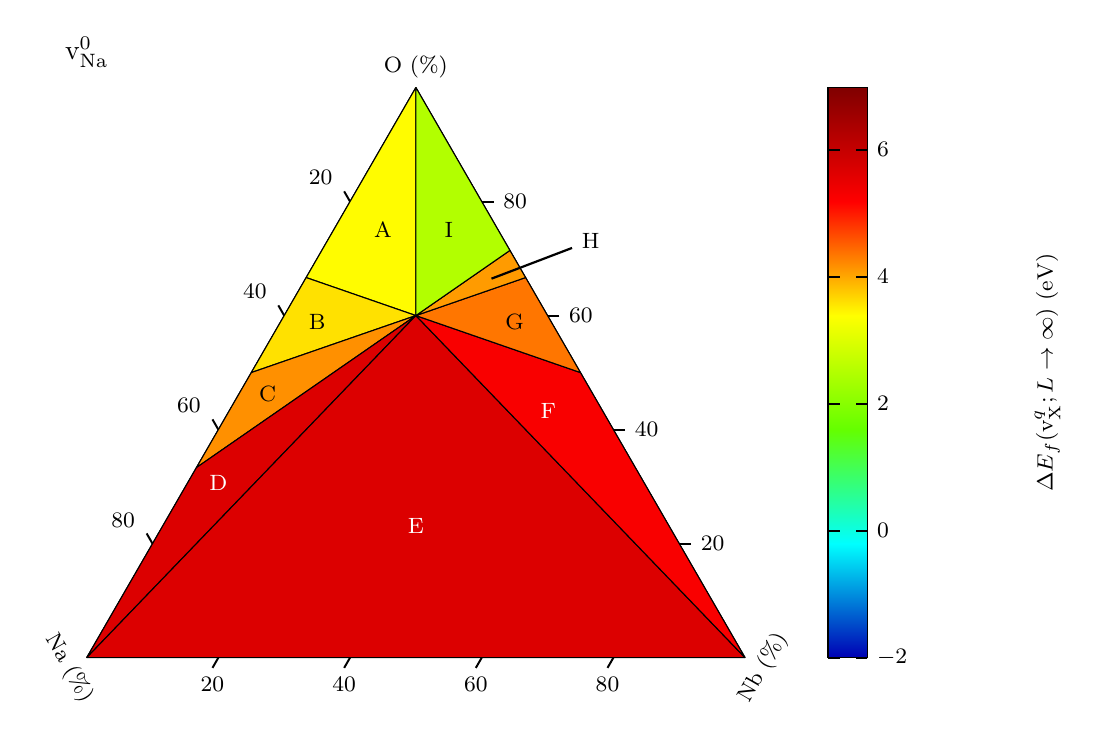
\begin{tikzpicture}
    \begin{ternaryaxis}[
        width=0.82\textwidth,
        xlabel=O ($\%$),
        xlabel style={%
            font=\footnotesize,
            at={(axis cs:1,0,0)},
            anchor=south
        },
        xtick={0.2,0.4,0.6,0.8},
        xticklabels={$20$,$40$,$60$,$80$},
        xticklabel style={font=\footnotesize},
        xtick style={line width=0.25mm, color=black},
        ylabel=Na ($\%$),
        ylabel style={%
            font=\footnotesize,
            at={(axis cs:0,1,0)},
            anchor=north,
            rotate=-60
        },
        ytick={0.2,0.4,0.6,0.8},
        yticklabels={$20$,$40$,$60$,$80$},
        yticklabel style={font=\footnotesize},
        ytick style={line width=0.25mm, color=black},
        zlabel=Nb ($\%$),
        zlabel style={%
            font=\footnotesize,
            at={(axis cs:0,0,1)},
            anchor=north,
            rotate=60
        },
        ztick={0.2,0.4,0.6,0.8},
        zticklabels={$20$,$40$,$60$,$80$},
        zticklabel style={font=\footnotesize},
        ztick style={line width=0.25mm, color=black},
        clip=false,
        no markers,
        colorbar,
        colormap/bluered,
        colorbar style={%
            ylabel=$\Delta E_f (\text{v}_{\ce{X}}^{q}; L\to\infty)$ (\si{\electronvolt}),
            ylabel style={
                font=\footnotesize,
                at={(axis description cs:5.0,0.5)}
            },
            yticklabel style={%
                font=\footnotesize,
                /pgf/number format/.cd,
                fixed,
                fixed zerofill,
                precision=0,
                /tikz/.cd
            },
            ytick style={line width=0.25mm, color=black},
        },
        point meta min=-2.0,
        of colormap/target pos min*=-2.0,
        point meta max=6.9814,
        of colormap/target pos max*=6.9814
    ]
        \addplot3 [patch, faceted color=black, point meta=\thisrow{H}] table {%
            O        Na       Nb       H
            1.0      0.0      0.0      3.4040
            0.6      0.2      0.2      3.4040
            0.666667 0.333333 0.0      3.4040
        };

        \addplot3 [patch, faceted color=black, point meta=\thisrow{H}] table {%
            O        Na       Nb       H
            0.666667 0.333333 0.0      3.5950
            0.6      0.2      0.2      3.5950
            0.5      0.5      0.0      3.5950
        };

        \addplot3 [patch, faceted color=black, point meta=\thisrow{H}] table {%
            O        Na       Nb       H
            0.5      0.5      0.0      4.1621
            0.6      0.2      0.2      4.1621
            0.333333 0.666667 0.0      4.1621
        };

        \addplot3 [patch, faceted color=black, point meta=\thisrow{H}] table {%
            O        Na       Nb       H
            0.333333 0.666667 0.0      5.6681
            0.6      0.2      0.2      5.6681
            0.0      1.0      0.0      5.6681
        };

        \addplot3 [patch, faceted color=black, point meta=\thisrow{H}] table {%
            O        Na       Nb       H
            0.0      1.0      0.0      5.6681
            0.6      0.2      0.2      5.6681
            0.0      0.0      1.0      5.6681
        };

        \addplot3 [patch, faceted color=black, point meta=\thisrow{H}] table {%
            O        Na       Nb       H
            0.0      0.0      1.0      5.2642
            0.6      0.2      0.2      5.2642
            0.5      0.0      0.5      5.2642
        };

        \addplot3 [patch, faceted color=black, point meta=\thisrow{H}] table {%
            O        Na       Nb       H
            0.5      0.0      0.5      4.3482
            0.6      0.2      0.2      4.3482
            0.666667 0.0      0.333333 4.3482
        };

        \addplot3 [patch, faceted color=black, point meta=\thisrow{H}] table {%
            O        Na       Nb       H
            0.714286 0.0      0.285714 4.0844
            0.6      0.2      0.2      4.0844
            0.666667 0.0      0.333333 4.0844
        };

        \addplot3 [patch, faceted color=black, point meta=\thisrow{H}] table {%
            O        Na       Nb       H
            0.714286 0.0      0.285714 2.4897
            0.6      0.2      0.2      2.4897
            1.0      0.0      0.0      2.4897
        };

        \node [] at (cartesian cs:0.450, 0.650) {\footnotesize A};
        \node [] at (cartesian cs:0.350, 0.510) {\footnotesize B};
        \node [] at (cartesian cs:0.275, 0.400) {\footnotesize C};
        \node [] at (cartesian cs:0.200, 0.265) {\footnotesize \textcolor{white}{D}};
        \node [] at (cartesian cs:0.500, 0.200) {\footnotesize \textcolor{white}{E}};
        \node [] at (cartesian cs:0.701, 0.375) {\footnotesize \textcolor{white}{F}};
        \node [] at (cartesian cs:0.650, 0.510) {\footnotesize G};
        \node [pin={[pin distance=7ex, pin edge={black, thick}]15:\footnotesize H}] at (cartesian cs:0.600, 0.570) {};
        \node [] at (cartesian cs:0.550, 0.650) {\footnotesize I};
        \node [] at (cartesian cs:0.000, 0.920) {v$_{\ce{Na}}^0$};
    \end{ternaryaxis}
\end{tikzpicture}

				\caption{Variação do $\Delta E_f (\text{v}_{\ce{Na}}^{0};\, L \to \infty)$ em função do equilíbrio químico.\label{fig:energy_vac_na0}}
			\end{figure}
		\end{column}
		\begin{column}{.5\textwidth}
			\begin{itemize}
				\item Mínimo de \SI{2.49}{\electronvolt} com eq. \ce{Nb2O5-NaNbO3-O} (I) $\to$ favorecimento em condições oxidantes;
				\begin{itemize}
					\item Problema de volatividade do \ce{Na}\footnote[frame]{\cite{acker_microstructure_2014}};
				\end{itemize}
				\item $\Delta E_f$ cresce com o caráter redutor;
			\end{itemize}
		\end{column}
	\end{columns}
\end{frame}
\begin{frame}{Energia de Formação: \texorpdfstring{v$_{\ce{O}}^{0}$}{vO0}}
	\begin{columns}
		\begin{column}{.5\textwidth}
			\begin{figure}[t]
				\centering
				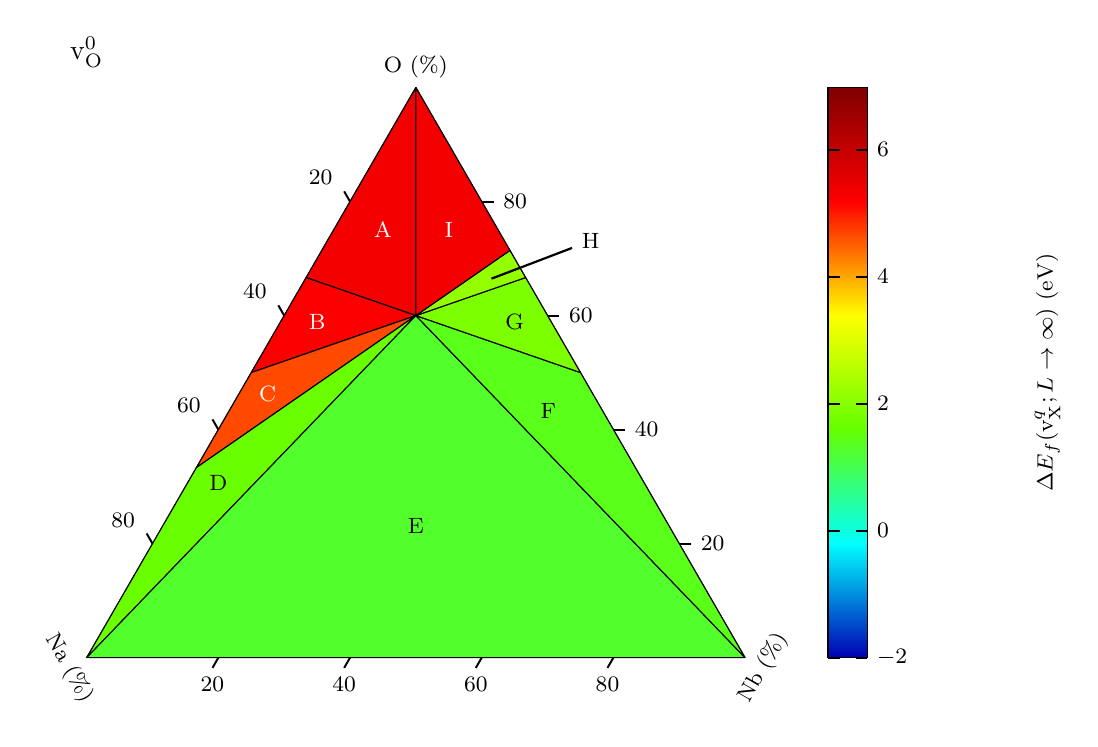
\begin{tikzpicture}
    \begin{ternaryaxis}[
        width=0.82\textwidth,
        xlabel=O ($\%$),
        xlabel style={%
            font=\footnotesize,
            at={(axis cs:1,0,0)},
            anchor=south
        },
        xtick={0.2,0.4,0.6,0.8},
        xticklabels={$20$,$40$,$60$,$80$},
        xticklabel style={font=\footnotesize},
        xtick style={line width=0.25mm, color=black},
        ylabel=Na ($\%$),
        ylabel style={%
            font=\footnotesize,
            at={(axis cs:0,1,0)},
            anchor=north,
            rotate=-60
        },
        ytick={0.2,0.4,0.6,0.8},
        yticklabels={$20$,$40$,$60$,$80$},
        yticklabel style={font=\footnotesize},
        ytick style={line width=0.25mm, color=black},
        zlabel=Nb ($\%$),
        zlabel style={%
            font=\footnotesize,
            at={(axis cs:0,0,1)},
            anchor=north,
            rotate=60
        },
        ztick={0.2,0.4,0.6,0.8},
        zticklabels={$20$,$40$,$60$,$80$},
        zticklabel style={font=\footnotesize},
        ztick style={line width=0.25mm, color=black},
        clip=false,
        no markers,
        colorbar,
        colormap/bluered,
        colorbar style={%
            ylabel=$\Delta E_f (\text{v}_{\ce{X}}^{q}; L\to\infty)$ (\si{\electronvolt}),
            ylabel style={
                font=\footnotesize,
                at={(axis description cs:5.0,0.5)}
            },
            yticklabel style={%
                font=\footnotesize,
                /pgf/number format/.cd,
                fixed,
                fixed zerofill,
                precision=0,
                /tikz/.cd
            },
            ytick style={line width=0.25mm, color=black},
        },
        point meta min=-2.0,
        of colormap/target pos min*=-2.0,
        point meta max=6.9814,
        of colormap/target pos max*=6.9814
    ]
        \addplot3 [patch, faceted color=black, point meta=\thisrow{H}] table {%
            O        Na       Nb       H
            1.0      0.0      0.0      5.3183
            0.6      0.2      0.2      5.3183
            0.666667 0.333333 0.0      5.3183
        };

        \addplot3 [patch, faceted color=black, point meta=\thisrow{H}] table {%
            O        Na       Nb       H
            0.666667 0.333333 0.0      5.2228
            0.6      0.2      0.2      5.2228
            0.5      0.5      0.0      5.2228
        };

        \addplot3 [patch, faceted color=black, point meta=\thisrow{H}] table {%
            O        Na       Nb       H
            0.5      0.5      0.0      4.6557
            0.6      0.2      0.2      4.6557
            0.333333 0.666667 0.0      4.6557
        };

        \addplot3 [patch, faceted color=black, point meta=\thisrow{H}] table {%
            O        Na       Nb       H
            0.333333 0.666667 0.0      1.6438
            0.6      0.2      0.2      1.6438
            0.0      1.0      0.0      1.6438
        };

        \addplot3 [patch, faceted color=black, point meta=\thisrow{H}] table {%
            O        Na       Nb       H
            0.0      1.0      0.0      1.2724
            0.6      0.2      0.2      1.2724
            0.0      0.0      1.0      1.2724
        };

        \addplot3 [patch, faceted color=black, point meta=\thisrow{H}] table {%
            O        Na       Nb       H
            0.0      0.0      1.0      1.4071
            0.6      0.2      0.2      1.4071
            0.5      0.0      0.5      1.4071
        };

        \addplot3 [patch, faceted color=black, point meta=\thisrow{H}] table {%
            O        Na       Nb       H
            0.5      0.0      0.5      1.8651
            0.6      0.2      0.2      1.8651
            0.666667 0.0      0.333333 1.8651
        };

        \addplot3 [patch, faceted color=black, point meta=\thisrow{H}] table {%
            O        Na       Nb       H
            0.714286 0.0      0.285714 2.1288
            0.6      0.2      0.2      2.1288
            0.666667 0.0      0.333333 2.1288
        };

        \addplot3 [patch, faceted color=black, point meta=\thisrow{H}] table {%
            O        Na       Nb       H
            0.714286 0.0      0.285714 5.3183
            0.6      0.2      0.2      5.3183
            1.0      0.0      0.0      5.3183
        };

        \node [] at (cartesian cs:0.450, 0.650) {\footnotesize\textcolor{white}{A}};
        \node [] at (cartesian cs:0.350, 0.510) {\footnotesize\textcolor{white}{B}};
        \node [] at (cartesian cs:0.275, 0.400) {\footnotesize\textcolor{white}{C}};
        \node [] at (cartesian cs:0.200, 0.265) {\footnotesize D};
        \node [] at (cartesian cs:0.500, 0.200) {\footnotesize E};
        \node [] at (cartesian cs:0.701, 0.375) {\footnotesize F};
        \node [] at (cartesian cs:0.650, 0.510) {\footnotesize G};
        \node [pin={[pin distance=7ex, pin edge={black, thick}]15:\footnotesize H}] at (cartesian cs:0.600, 0.570) {};
        \node [] at (cartesian cs:0.550, 0.650) {\footnotesize\textcolor{white}{I}};
        \node [] at (cartesian cs:0.000, 0.920) {v$_{\ce{O}}^0$};
    \end{ternaryaxis}
\end{tikzpicture}

				\caption{Variação do $\Delta E_f (\text{v}_{\ce{O}}^{0};\, L \to \infty)$ em função do equilíbrio químico.\label{fig:energy_vac_o0}}
			\end{figure}
		\end{column}
		\begin{column}{.5\textwidth}
			\begin{itemize}
				\item Mínimo de \SI{1.27}{\electronvolt} com equilíbrio \ce{Na-NaNbO3-Nb} (E) $\to$ favorecimento em condições redutoras;
				\item $\Delta E_f$ cresce com o caráter oxidante;
			\end{itemize}
			\begin{center}
				\alert{Ambientes mais redutores que em C e H favorecem v$_{\ce{O}}^{0}$ em detrimento de v$_{\ce{Na}}^{0}$!}
			\end{center}
		\end{column}
	\end{columns}
\end{frame}
\begin{frame}{Energia de Formação: \texorpdfstring{v$_{\ce{Na}}^{1-}$}{vNa1-}}
	\begin{columns}
		\begin{column}{.5\textwidth}
			\begin{figure}[t]
				\centering
				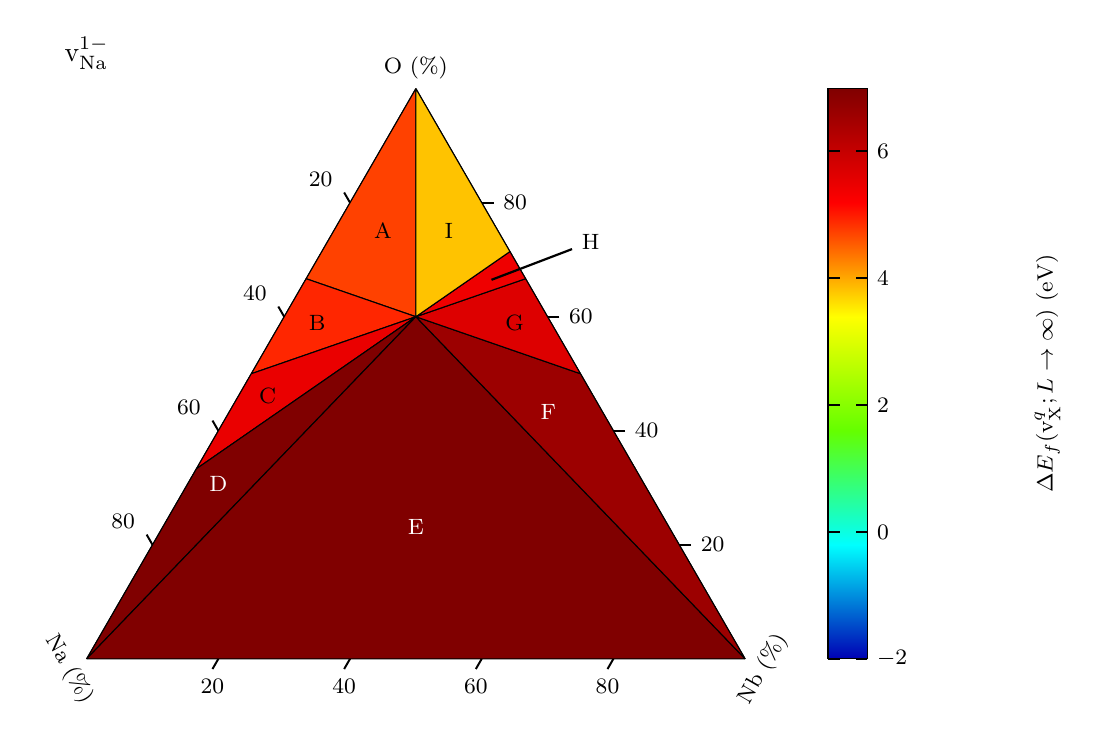
\begin{tikzpicture}
    \begin{ternaryaxis}[
        width=0.82\textwidth,
        xlabel=O ($\%$),
        xlabel style={%
            font=\footnotesize,
            at={(axis cs:1,0,0)},
            anchor=south
        },
        xtick={0.2,0.4,0.6,0.8},
        xticklabels={$20$,$40$,$60$,$80$},
        xticklabel style={font=\footnotesize},
        xtick style={line width=0.25mm, color=black},
        ylabel=Na ($\%$),
        ylabel style={%
            font=\footnotesize,
            at={(axis cs:0,1,0)},
            anchor=north,
            rotate=-60
        },
        ytick={0.2,0.4,0.6,0.8},
        yticklabels={$20$,$40$,$60$,$80$},
        yticklabel style={font=\footnotesize},
        ytick style={line width=0.25mm, color=black},
        zlabel=Nb ($\%$),
        zlabel style={%
            font=\footnotesize,
            at={(axis cs:0,0,1)},
            anchor=north,
            rotate=60
        },
        ztick={0.2,0.4,0.6,0.8},
        zticklabels={$20$,$40$,$60$,$80$},
        zticklabel style={font=\footnotesize},
        ztick style={line width=0.25mm, color=black},
        clip=false,
        no markers,
        colorbar,
        colormap/bluered,
        colorbar style={%
            ylabel=$\Delta E_f (\text{v}_{\ce{X}}^{q}; L\to\infty)$ (\si{\electronvolt}),
            ylabel style={
                font=\footnotesize,
                at={(axis description cs:5.0,0.5)}
            },
            yticklabel style={%
                font=\footnotesize,
                /pgf/number format/.cd,
                fixed,
                fixed zerofill,
                precision=0,
                /tikz/.cd
            },
            ytick style={line width=0.25mm, color=black},
        },
        point meta min=-2.0,
        of colormap/target pos min*=-2.0,
        point meta max=6.9814,
        of colormap/target pos max*=6.9814
    ]
        \addplot3 [patch, faceted color=black, point meta=\thisrow{H}] table {%
            O        Na       Nb       H
            1.0      0.0      0.0      4.7173
            0.6      0.2      0.2      4.7173
            0.666667 0.333333 0.0      4.7173
        };

        \addplot3 [patch, faceted color=black, point meta=\thisrow{H}] table {%
            O        Na       Nb       H
            0.666667 0.333333 0.0      4.9083
            0.6      0.2      0.2      4.9083
            0.5      0.5      0.0      4.9083
        };

        \addplot3 [patch, faceted color=black, point meta=\thisrow{H}] table {%
            O        Na       Nb       H
            0.5      0.5      0.0      5.4754
            0.6      0.2      0.2      5.4754
            0.333333 0.666667 0.0      5.4754
        };

        \addplot3 [patch, faceted color=black, point meta=\thisrow{H}] table {%
            O        Na       Nb       H
            0.333333 0.666667 0.0      6.9814
            0.6      0.2      0.2      6.9814
            0.0      1.0      0.0      6.9814
        };

        \addplot3 [patch, faceted color=black, point meta=\thisrow{H}] table {%
            O        Na       Nb       H
            0.0      1.0      0.0      6.9814
            0.6      0.2      0.2      6.9814
            0.0      0.0      1.0      6.9814
        };

        \addplot3 [patch, faceted color=black, point meta=\thisrow{H}] table {%
            O        Na       Nb       H
            0.0      0.0      1.0      6.5775
            0.6      0.2      0.2      6.5775
            0.5      0.0      0.5      6.5775
        };

        \addplot3 [patch, faceted color=black, point meta=\thisrow{H}] table {%
            O        Na       Nb       H
            0.5      0.0      0.5      5.6615
            0.6      0.2      0.2      5.6615
            0.666667 0.0      0.333333 5.6615
        };

        \addplot3 [patch, faceted color=black, point meta=\thisrow{H}] table {%
            O        Na       Nb       H
            0.714286 0.0      0.285714 5.3977
            0.6      0.2      0.2      5.3977
            0.666667 0.0      0.333333 5.3977
        };

        \addplot3 [patch, faceted color=black, point meta=\thisrow{H}] table {%
            O        Na       Nb       H
            0.714286 0.0      0.285714 3.8030
            0.6      0.2      0.2      3.8030
            1.0      0.0      0.0      3.8030
        };

        \node [] at (cartesian cs:0.450, 0.650) {\footnotesize A};
        \node [] at (cartesian cs:0.350, 0.510) {\footnotesize B};
        \node [] at (cartesian cs:0.275, 0.400) {\footnotesize C};
        \node [] at (cartesian cs:0.200, 0.265) {\footnotesize \textcolor{white}{D}};
        \node [] at (cartesian cs:0.500, 0.200) {\footnotesize \textcolor{white}{E}};
        \node [] at (cartesian cs:0.701, 0.375) {\footnotesize \textcolor{white}{F}};
        \node [] at (cartesian cs:0.650, 0.510) {\footnotesize G};
        \node [pin={[pin distance=7ex, pin edge={black, thick}]15:\footnotesize H}] at (cartesian cs:0.600, 0.570) {};
        \node [] at (cartesian cs:0.550, 0.650) {\footnotesize I};
        \node [] at (cartesian cs:0.000, 0.920) {v$_{\ce{Na}}^{1-}$};
    \end{ternaryaxis}
\end{tikzpicture}

				\caption{Variação do $\Delta E_f (\text{v}_{\ce{Na}}^{1-};\, L \to \infty)$ em função do equilíbrio químico.\label{fig:energy_vac_na1}}
			\end{figure}
		\end{column}
		\begin{column}{.5\textwidth}
			\begin{itemize}
				\item Mínimo de \SI{3.80}{\electronvolt} com eq. \ce{Nb2O5-NaNbO3-O} (I) $\to$ favorecimento em condições oxidantes;
				\item $\Delta E_f (\text{v}_{\ce{Na}}^{1-}) > \Delta E_f (\text{v}_{\ce{Na}}^{0}) \to$ formação do defeito pontual neutro;
			\end{itemize}
		\end{column}
	\end{columns}
\end{frame}
\begin{frame}{Energia de Formação: \texorpdfstring{v$_{\ce{O}}^{2+}$}{vO2+} I}
	\begin{columns}
		\begin{column}{.5\textwidth}
			\begin{figure}[t]
				\centering
				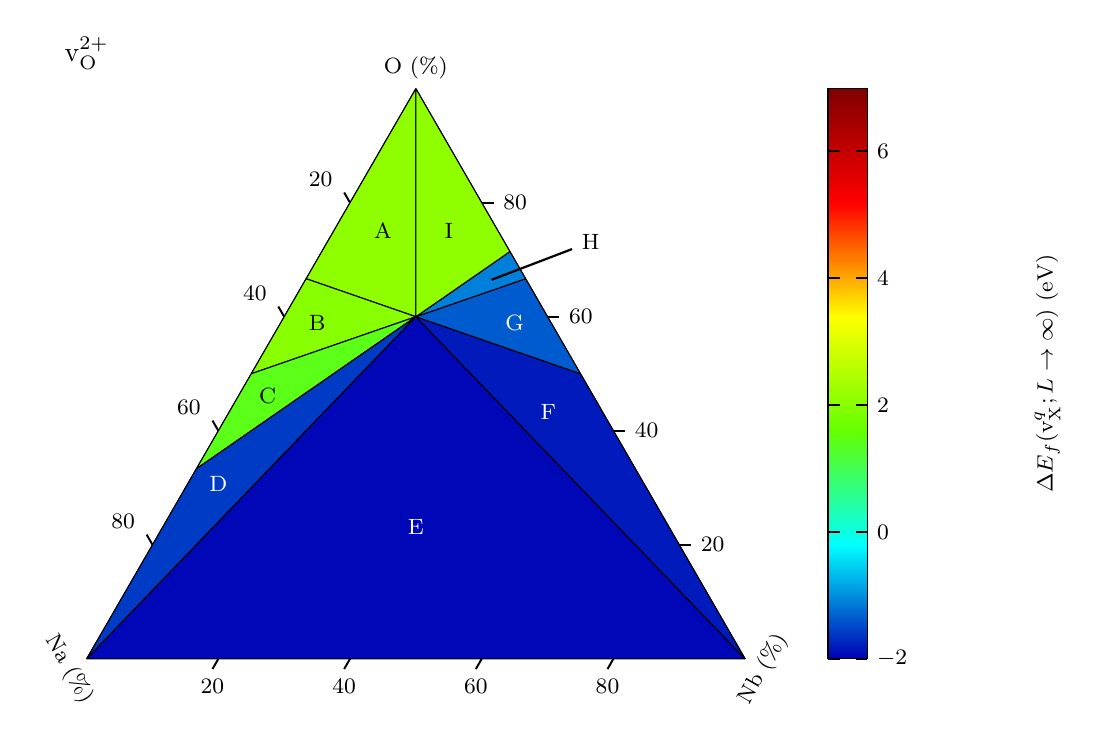
\begin{tikzpicture}
    \begin{ternaryaxis}[
        width=.82\textwidth,
        xlabel=O ($\%$),
        xlabel style={%
            font=\footnotesize,
            at={(axis cs:1,0,0)},
            anchor=south
        },
        xtick={0.2,0.4,0.6,0.8},
        xticklabels={$20$,$40$,$60$,$80$},
        xticklabel style={font=\footnotesize},
        xtick style={line width=0.25mm, color=black},
        ylabel=Na ($\%$),
        ylabel style={%
            font=\footnotesize,
            at={(axis cs:0,1,0)},
            anchor=north,
            rotate=-60
        },
        ytick={0.2,0.4,0.6,0.8},
        yticklabels={$20$,$40$,$60$,$80$},
        yticklabel style={font=\footnotesize},
        ytick style={line width=0.25mm, color=black},
        zlabel=Nb ($\%$),
        zlabel style={%
            font=\footnotesize,
            at={(axis cs:0,0,1)},
            anchor=north,
            rotate=60
        },
        ztick={0.2,0.4,0.6,0.8},
        zticklabels={$20$,$40$,$60$,$80$},
        zticklabel style={font=\footnotesize},
        ztick style={line width=0.25mm, color=black},
        clip=false,
        no markers,
        colorbar,
        colormap/bluered,
        colorbar style={%
            ylabel=$\Delta E_f (\text{v}_{\ce{X}}^{q}; L\to\infty)$ (\si{\electronvolt}),
            ylabel style={
                font=\footnotesize,
                at={(axis description cs:5.0,0.5)}
            },
            yticklabel style={%
                font=\footnotesize,
                /pgf/number format/.cd,
                fixed,
                fixed zerofill,
                precision=0,
                /tikz/.cd
            },
            ytick style={line width=0.25mm, color=black},
        },
        point meta min=-2.0,
        of colormap/target pos min*=-2.0,
        point meta max=6.9814,
        of colormap/target pos max*=6.9814
    ]
        \addplot3 [patch, faceted color=black, point meta=\thisrow{H}] table {%
            O        Na       Nb       H
            1.0      0.0      0.0      2.0927
            0.6      0.2      0.2      2.0927
            0.666667 0.333333 0.0      2.0927
        };

        \addplot3 [patch, faceted color=black, point meta=\thisrow{H}] table {%
            O        Na       Nb       H
            0.666667 0.333333 0.0      1.9972
            0.6      0.2      0.2      1.9972
            0.5      0.5      0.0      1.9972
        };

        \addplot3 [patch, faceted color=black, point meta=\thisrow{H}] table {%
            O        Na       Nb       H
            0.5      0.5      0.0      1.4301
            0.6      0.2      0.2      1.4301
            0.333333 0.666667 0.0      1.4301
        };

        \addplot3 [patch, faceted color=black, point meta=\thisrow{H}] table {%
            O        Na       Nb       H
            0.333333 0.666667 0.0      -1.5818
            0.6      0.2      0.2      -1.5818
            0.0      1.0      0.0      -1.5818
        };

        \addplot3 [patch, faceted color=black, point meta=\thisrow{H}] table {%
            O        Na       Nb       H
            0.0      1.0      0.0      -1.9532
            0.6      0.2      0.2      -1.9532
            0.0      0.0      1.0      -1.9532
        };

        \addplot3 [patch, faceted color=black, point meta=\thisrow{H}] table {%
            O        Na       Nb       H
            0.0      0.0      1.0      -1.8185
            0.6      0.2      0.2      -1.8185
            0.5      0.0      0.5      -1.8185
        };

        \addplot3 [patch, faceted color=black, point meta=\thisrow{H}] table {%
            O        Na       Nb       H
            0.5      0.0      0.5      -1.3605
            0.6      0.2      0.2      -1.3605
            0.666667 0.0      0.333333 -1.3605
        };

        \addplot3 [patch, faceted color=black, point meta=\thisrow{H}] table {%
            O        Na       Nb       H
            0.714286 0.0      0.285714 -1.0968
            0.6      0.2      0.2      -1.0968
            0.666667 0.0      0.333333 -1.0968
        };

        \addplot3 [patch, faceted color=black, point meta=\thisrow{H}] table {%
            O        Na       Nb       H
            0.714286 0.0      0.285714 2.0927
            0.6      0.2      0.2      2.0927
            1.0      0.0      0.0      2.0927
        };

        \node [] at (cartesian cs:0.450, 0.650) {\footnotesize A};
        \node [] at (cartesian cs:0.350, 0.510) {\footnotesize B};
        \node [] at (cartesian cs:0.275, 0.400) {\footnotesize C};
        \node [] at (cartesian cs:0.200, 0.265) {\footnotesize\textcolor{white}{D}};
        \node [] at (cartesian cs:0.500, 0.200) {\footnotesize\textcolor{white}{E}};
        \node [] at (cartesian cs:0.701, 0.375) {\footnotesize\textcolor{white}{F}};
        \node [] at (cartesian cs:0.650, 0.510) {\footnotesize\textcolor{white}{G}};
        \node [pin={[pin distance=7ex, pin edge={black, thick}]15:\footnotesize H}] at (cartesian cs:0.600, 0.570) {};
        \node [] at (cartesian cs:0.550, 0.650) {\footnotesize I};
        \node [] at (cartesian cs:0.000, 0.920) {v$_{\ce{O}}^{2+}$};
    \end{ternaryaxis}
\end{tikzpicture}

				\caption{Variação do $\Delta E_f (\text{v}_{\ce{O}}^{2+};\, L \to \infty)$ em função do equilíbrio químico.\label{fig:energy_vac_o2}}
			\end{figure}
		\end{column}
		\begin{column}{.5\textwidth}
			\begin{itemize}
				\item Mínimo de \SI{-1.95}{\electronvolt} com equilíbrio \ce{Na-NaNbO3-Nb} (E) $\to$ favorecimento em condições redutoras;
				\item $\Delta E_f (\text{v}_{\ce{O}}^{2+}) << \Delta E_f (\text{v}_{\ce{O}}^{0}) \to$ formação do defeito pontual ionizado;
				\item \alert{Energias de formação negativas para equilíbrios químicos entre D e H;}
			\end{itemize}
		\end{column}
	\end{columns}
\end{frame}
\begin{frame}{Energia de Formação: \texorpdfstring{v$_{\ce{O}}^{2+}$}{vO2+} II}
	\begin{itemize}
		\item $\Delta E_f (\text{v}_{\ce{O}}^{2+}; L) < 0$ para os três tamanhos de supercélula $\to$ $\Delta E_f (\text{v}_{\ce{O}}^{2+}; L \to \infty) < 0$;
		\item Fatores:
		\begin{itemize}
			\item $E_T (\text{v}_{\ce{O}}^{2+}; L) - E_T (\text{perfeito}; L) > 0$ para $1\times1\times1$, $2\times2\times2$ e $3\times3\times3$;
			\item $E_T (\text{v}_{\ce{O}}^{2+}; L) - E_T (\text{perfeito}; L) + q \varepsilon_F > 0$ para todas as supercélulas;
			\item $E_T (\text{v}_{\ce{O}}^{2+}; L) - E_T (\text{perfeito}; L) + q \varepsilon_F < | \mu_{\ce{O}} |$ para os equilíbrios D à H;
		\end{itemize}
		\item Hipótese: $E_T (\text{v}_{\ce{O}}^{2+}; L) - E_T (\text{perfeito}; L)$ ou $ q \varepsilon_F$ subestimados $\to$ troca com reservatório $e^{-}$ depende do tamanho de banda proibida;
		\begin{itemize}
			\item $q \varepsilon_F$ da banda proibida experimental\footnote[frame]{\cite{li_constructing_2014}} (\SI{3.42}{\electronvolt}) dá $\Delta E_f (\text{v}_{\ce{O}}^{2+}; L \to \infty) = \SI{0.08}{\electronvolt}$ $\to$ melhor descrição da banda proibida pode melhorar a descrição de v$_{\ce{O}}^{2+}$;
			\item Modelo de v$_{\ce{O}}^{2+}$ isolado? Modelo com um defeito de Schottky/Frenkel?
		\end{itemize}\vfill
		\begin{equation*}
			\Delta E_f (\text{v}_{\ce{X}}^{q}; L) = E_T (\text{v}_{\ce{X}}^{q}; L) - E_T (\text{perfeito}; L) - n_{\ce{X}} \mu_{\ce{X}} + q \varepsilon_F + E_c
		\end{equation*}
	\end{itemize}
\end{frame}

\subsection{Filme Fino De \texorpdfstring{\ce{NaNbO3}}{NaNbO3} Orientado Em \texorpdfstring{$[100]$}{[100]}}
\begin{frame}{Reconfiguração Cristalina}
	\begin{columns}
		\begin{column}{.4\textwidth}
			\begin{figure}[t]
				\centering
				%! TeX root = ../root/root.tex 
\begin{tikzpicture}[remember picture, baseline=-.5ex]
    \draw (0.00cm, 0.00cm) node {
        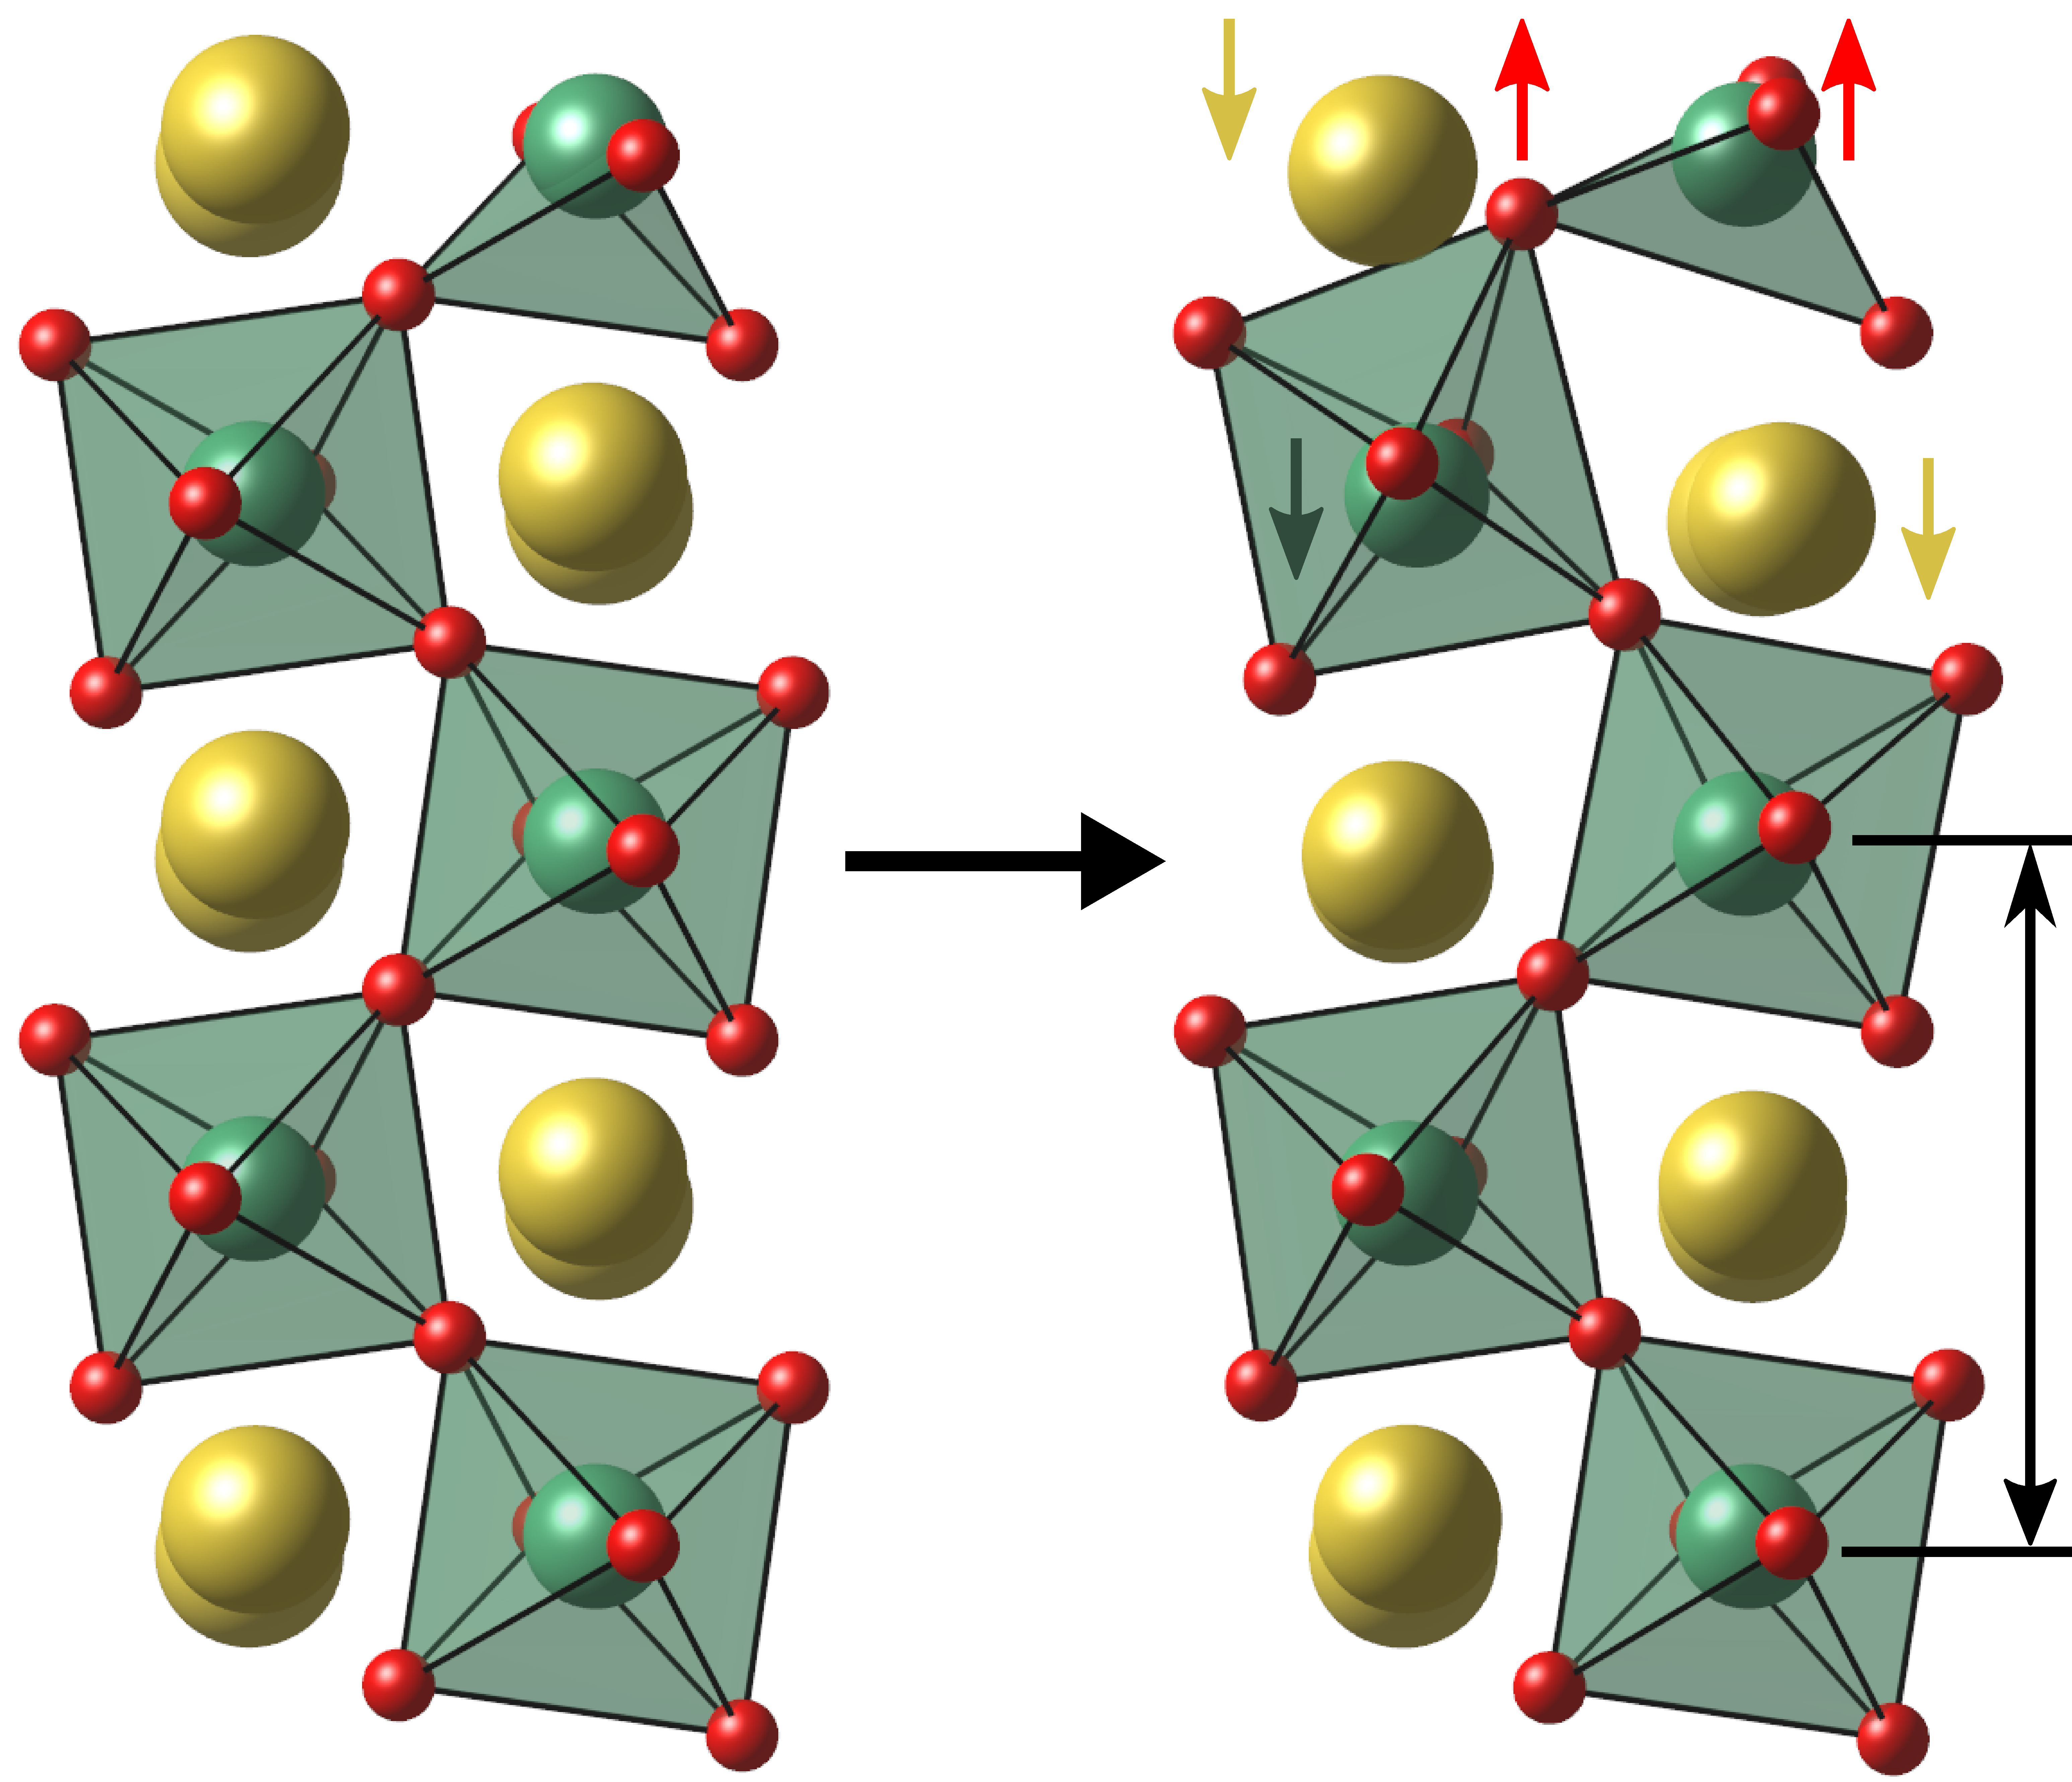
\includegraphics[width=0.85\linewidth]{../floats/tf_rlx/bulk-to-tf.pdf}
    };
    \draw (2.10cm, 1.75cm) node [coordinate] (n1) {};
    \draw (2.20cm, 1.00cm) node [coordinate] (n2) {};
    \draw (2.35cm,-0.75cm) node [coordinate] (n3) {};
\end{tikzpicture}
				\caption{Metade superior do filme fino antes (esquerda) e depois (direita) de relaxar mostrando o deslocamento atômico.\label{fig:slabs_relax}}
			\end{figure}
			\[\scriptstyle{P_L = \frac{\langle \theta \rangle}{\SI{180}{\degree}};\,\Delta_d = \frac{1}{6} \sum^{6}_{i=1} \frac{|d_i - \langle d \rangle|}{\langle d \rangle}}\]
		\end{column}
		\begin{column}{.45\textwidth}
		Energia total mínima com parâmetros de rede $b$ e $c$ \SI{1}{\percent} maiores que os do cristal volumoso.
			\begin{block}{Superfície}
				\begin{itemize}
					\item \tikz[remember picture,overlay]{\node [anchor=west, left=0.7cm] (t1) {};}Planaridade $P_L = \SI{75}{\percent}$;
					\item Ligação \ce{Nb-O} diminui \SI{2.2}{\percent};
				\end{itemize}
			\end{block}
			\begin{block}{Subsuperfície}
				\begin{itemize}
					\item \tikz[remember picture,overlay]{\node [anchor=west, left=0.7cm] (t2) {};}Índice de deformação $\Delta_d = \SI{6}{\percent}$;
					\item Ligação \ce{Nb-O} aumenta \SI{2.3}{\percent};
				\end{itemize}
			\end{block}
			\begin{block}{Interna}
				\begin{itemize}
					\item \tikz[remember picture,overlay]{\node [anchor=west, left=0.7cm] (t3) {};}Índice de deformação: $\Delta_d = \SI{3}{\percent}$;
					\item Ligação \ce{Nb-O} $\approxeq$ do cristal volumoso ($+\SI{1.0}{\percent}$);
				\end{itemize}
			\end{block}
		\end{column}
	\end{columns}
	\begin{tikzpicture}[remember picture,overlay]
		\path (n1) edge [arrow, out=0, in=180] (t1);
		\path (n2) edge [arrow, out=0, in=180] (t2);
		\path (n3) edge [arrow, out=300, in=180] (t3);
	\end{tikzpicture}
\end{frame}
\begin{frame}{Reconfiguração Espacial Dos e$^-$}
	\begin{columns}
		\begin{column}{.6\textwidth}
			\begin{figure}[t]
				\centering
				\input{../floats/charge_layer/charge_layer.pdf_tex}
				\caption{Mudança do total de cargas de \ce{Nb} no filme fino em referência ao total de cargas de \ce{Nb} no cristal volumoso.\label{fig:bader_chg_comparison}}
			\end{figure}
		\end{column}
		\begin{column}{.4\textwidth}
			\begin{itemize}
				\item Elétrons no \ce{Nb} de superfície: $6 + 2,\!92$;
				\item \ce{Nb} mais internos também ganharam elétrons $\to$ \alert{rearranjo atômico + metalização};
			\end{itemize}
		\end{column}
	\end{columns}
\end{frame}
\begin{frame}{Densidade De Estados Projetada}
	\begin{columns}
		\begin{column}{.5\textwidth}
			\begin{figure}[t]
				\centering
				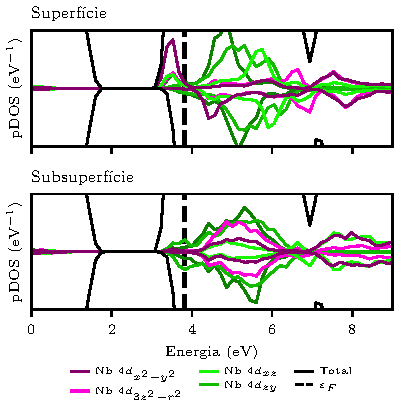
\includegraphics{../floats/pdos_nn_tf/pdos_nn_thinfilm_surface_subsurface.pdf}
				\caption{pDOS destacando a resposta da superfície e subsuperfície. Linha tracejada marca o nível de Fermi.\label{fig:pdosNblayer}}
			\end{figure}
		\end{column}
		\begin{column}{.5\textwidth}
			\begin{itemize}
				\item \alert{Camadas superficiais induzem polarização de \textit{spin} e metalização!}
				\item Diferença entre \textit{spins} $\uparrow$ e $\downarrow$ de \SI{1.75}{\electronvolt}, momento magnético de $3,\!95\,\mu_B$;
				\begin{itemize}
					\item \ce{Nb} de superfície com $0,\!99\,\mu_B/\text{át.}$;
				\end{itemize}
				\item Valência comparável ao cristal volumoso;
				\item Parte inferior da condução dominada por níveis de superfície;
				\item Quebra de 2 \ce{Nb-O} estabilizam orbitais \ce{Nb} $4d$ da superfície;
				\item Deformação do \ce{NbO6} na subsuperfície afeta menos os \ce{Nb} $4d$;
			\end{itemize}
		\end{column}
	\end{columns}
\end{frame}

\subsection{Tensão Biaxial No \texorpdfstring{\ce{NaNbO3}}{NaNbO3}}
\begin{frame}{Propriedades Da Rede Cristalina}
	\begin{itemize}
		\item Compressão reduz a planaridade do \ce{NbO4} e aumenta a deformação do \ce{NbO6} $\to$ piora sobreposição $p - d$;
		\item Tração aumenta a planaridade do \ce{NbO4} e diminui a deformação do \ce{NbO6} $\to$ melhora sobreposição $p - d$;
	\end{itemize}
	\begin{figure}[b]
		\centering
		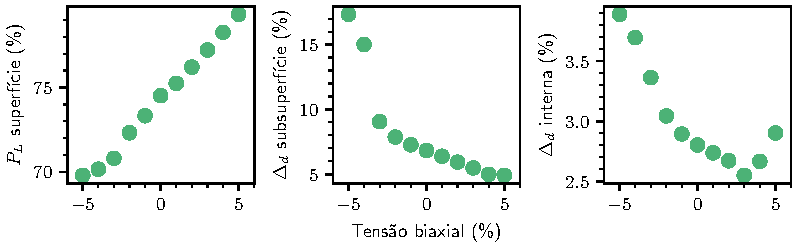
\includegraphics{../floats/geometry_evo/nn_pl_baur_strain_evolution.pdf}
		\caption{Geometria dos \ce{NbO4} de superfície (a) e \ce{NbO6} de subsuperfície (2º) e região interna (3º).\label{fig:geo_evo_nn}}
	\end{figure}
	\begin{equation*}
		\scriptstyle{P_L = \frac{\theta}{\SI{180}{\degree}};\; \Delta_d = \frac{1}{6} \sum^{6}_{i=1} \frac{|d_{\ce{Nb-O}\, i} - \overline{d_{\ce{Nb-O}}}|}{\overline{d_{\ce{Nb-O}}}};}
	\end{equation*}
\end{frame}
\begin{frame}{Distribuição De e$^-$}
	\begin{columns}
		\begin{column}{.65\textwidth}
			\begin{figure}[t]
				\centering
				\input{../floats/charge_evo/bader_strain_evolution_nn.pdf_tex}
				\caption{Realocação de cargas através do filme fino com a tensão biaxial.\label{fig:bader_strain_evolution}}
			\end{figure}
		\end{column}
		\begin{column}{.35\textwidth}
		\begin{itemize}
			\item Compressão: elétrons \ce{Nb} superfície $\Rightarrow$ \ce{Nb} subsuperfície;
			\item Tração: elétrons \ce{Nb} subsuperfície $\Rightarrow$ \ce{Nb} superfície;
		\end{itemize}	
		\end{column}
	\end{columns}
\end{frame}
\begin{frame}{Estrutura De Bandas: Tração}
	\begin{columns}
		\begin{column}{.6\textwidth}
			\begin{figure}[t]
				\centering
				\input{../floats/band_structure_evo_tf_nn/bndstr-pdos_NNO_t5.pdf_tex}
				\caption{Bandas em estado fundamental ($\epsilon = 1\%$) e em tração ($5\%$).\label{fig:bnd_str_tf_nn_t5}}
			\end{figure}
		\end{column}
		\begin{column}{.4\textwidth}
			\begin{itemize}
				\item Alinhamento em relação ao cristal volumoso;
				\item Níveis de superfície $\to$ elétrons desemparelhados;
				\item Tração \alert{diminuiu}:
				\begin{itemize}
					\item Tamanho da banda proibida;
					\item Nível dos estados de superfície $\to$ adentraram a banda proibida;
				\end{itemize}
				\item Deformação dos \ce{NbO4} de superfície e \ce{NbO6} de subsuperfície $\to$ orbitais $p-d$ se afastam $\to$ níveis energéticos diminuíram $\to$ densidade de carga da superfície transferida para subsuperfície;
			\end{itemize}		
		\end{column}
	\end{columns}
\end{frame}
\begin{frame}{Estrutura De Bandas: Compressão}
	\begin{columns}
		\begin{column}{.6\textwidth}
			\begin{figure}[t]
				\centering
				\input{../floats/band_structure_evo_tf_nn/bndstr-pdos_NNO_c5.pdf_tex}
				\caption{Bandas em estado fundamental ($\epsilon = 1\%$) e em compressão ($-5\%$).\label{fig:bnd_str_tf_nn_c5}}
			\end{figure}
		\end{column}
		\begin{column}{.4\textwidth}
			\begin{itemize}
				\item Níveis de superfície $\to$ elétrons (continuam) desemparelhados;
				\item Bandas reagem de maneira \alert{oposta} à tração;
				\item Filme fino continua metalizado $\to$ provável inatividade catalítica;
				\item Proposta: defeitos de superfície, outras terminações;
			\end{itemize}
		\end{column}
	\end{columns}
\end{frame}

\subsection{Comparação Com o Filme Fino De \texorpdfstring{\ce{NaTaO3}}{NaTaO3}}
\begin{frame}{\texorpdfstring{\ce{NaNbO3}}{NaNbO3} \textit{vs.} \texorpdfstring{\ce{NaTaO3}}{NaTaO3}: Estado Fundamental}
	\begin{columns}
		\begin{column}{0.166666667\textwidth}
			\begin{tabular}{l}
				\toprule
				\multicolumn{1}{c}{\ce{NaNbO3}}\\\midrule
				\multicolumn{1}{c}{Superfície}\\
				$\Delta \overline{d_{\ce{Nb-O}}} = \SI{-2.2}{\percent}$\tikz[remember picture,overlay]{\node [anchor=east, shift={(4mm, 1.5mm)}] (lista_nb1) {};}\\
				$P_L = \SI{75}{\percent}$\\\midrule
				\multicolumn{1}{c}{Subsuperfície}\\
				$\Delta \overline{d_{\ce{Nb-O}}} = \SI{+2.5}{\percent}$\tikz[remember picture,overlay]{\node [anchor=east, shift={(4mm, 1.5mm)}] (lista_nb2) {};}\\
				$\Delta_d = \SI{6}{\percent}$\\\midrule
				\multicolumn{1}{c}{Interna}\\
				$\Delta \overline{d_{\ce{Nb-O}}} = \SI{+1.0}{\percent}$\tikz[remember picture,overlay]{\node [anchor=east, shift={(4mm, 1.5mm)}] (lista_nb3) {};}\\
				$\Delta_d = \SI{3}{\percent}$\\\bottomrule
			\end{tabular}
		\end{column}\hspace{5mm}
		\begin{column}{0.333333333\textwidth}
			\begin{figure}
				\centering
				%! TeX root = ../root/root.tex 
\begin{tikzpicture}[remember picture, baseline=-.5ex]
    \draw (0.00cm, 0.00cm) node {
        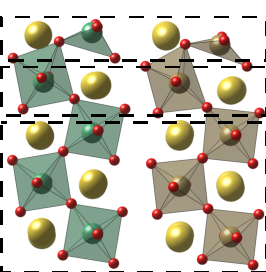
\includegraphics{../floats/nn_nt_tf_rlx/thin_film_nn_nt.pdf}
    };
    \draw (23mm,   16mm) node [coordinate] (nt1) {};
    \draw (23mm,    8mm) node [coordinate] (nt2) {};
    \draw (23mm,  -10mm) node [coordinate] (nt3) {};
    \draw (-23mm,  16mm) node [coordinate] (nb1) {};
    \draw (-23mm,   8mm) node [coordinate] (nb2) {};
    \draw (-23mm, -10mm) node [coordinate] (nb3) {};
\end{tikzpicture}

				\caption{Propriedades da estrutura cristalina dos filmes finos de \ce{NaNbO3} (esquerda) e \ce{NaTaO3} (direita).\label{fig:thin_film_nn_nt}}
			\end{figure}
		\end{column}
		\begin{column}{0.166666667\textwidth}
			\begin{tabular}{l}
				\toprule
				\multicolumn{1}{c}{\ce{NaTaO3}}\\\midrule
				\multicolumn{1}{c}{Superfície}\\
				\tikz[remember picture,overlay]{\node [anchor=west, shift={(-3.5mm, 1.5mm)}] (lista_nt1) {};}$\Delta \overline{d_{\ce{Ta-O}}} = \SI{-2.3}{\percent}$\\
				$P_L = \SI{84}{\percent}$\\\midrule
				\multicolumn{1}{c}{Subsuperfície}\\
				\tikz[remember picture,overlay]{\node [anchor=west, shift={(-3.5mm, 1.5mm)}] (lista_nt2) {};}$\Delta \overline{d_{\ce{Ta-O}}} = \SI{+2.1}{\percent}$\\
				$\Delta_d = \SI{3}{\percent}$\\\midrule
				\multicolumn{1}{c}{Interna}\\
				\tikz[remember picture,overlay]{\node [anchor=west, shift={(-3.5mm, 1.5mm)}] (lista_nt3) {};}$\Delta \overline{d_{\ce{Ta-O}}} = \SI{-0.1}{\percent}$\\
				$\Delta_d = \SI{0.3}{\percent}$\\\bottomrule
			\end{tabular}
		\end{column}\hspace{5mm}
	\end{columns}
	\begin{tikzpicture}[remember picture,overlay]
		\path (nt1) edge [arrow, out=0, in=180] (lista_nt1);
		\path (nt2) edge [arrow, out=0, in=180] (lista_nt2);
		\path (nt3) edge [arrow, out=0, in=180] (lista_nt3);
		\path (nb1) edge [arrow, out=180, in=0] (lista_nb1);
		\path (nb2) edge [arrow, out=180, in=0] (lista_nb2);
		\path (nb3) edge [arrow, out=180, in=0] (lista_nb3);
	\end{tikzpicture}
	\begin{equation*}
		\scriptstyle{P_L = \frac{\theta}{\SI{180}{\degree}};\; \Delta_d = \frac{1}{6} \sum^{6}_{i=1} \frac{|d_{\ce{Nb-O}\, i} - \overline{d_{\ce{Nb-O}}}|}{\overline{d_{\ce{Nb-O}}}};}
	\end{equation*}
\end{frame}
\begin{frame}{\texorpdfstring{\ce{NaNbO3}}{NaNbO3} \textit{vs.} \texorpdfstring{\ce{NaTaO3}}{NaTaO3}: Densidade de Estados}
	\begin{columns}
		\begin{column}{.5\textwidth}
			\begin{figure}[t]
				\centering
				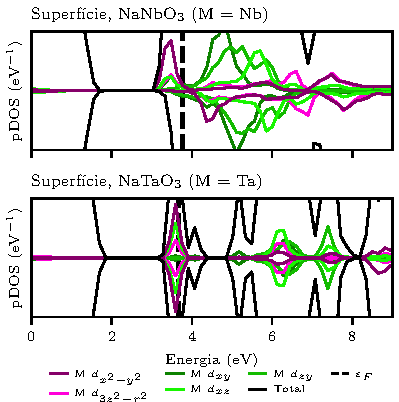
\includegraphics{../floats/pdos_nn_nt_tf/pdos_rlx_nn_nt_surface.pdf}
				\caption{DOS projetada dos filmes finos em estado fundamental.\label{fig:pdos_rlx_nn_nt_surface}}
			\end{figure}	
		\end{column}
		\begin{column}{.5\textwidth}
			\begin{itemize}
				\item Mesma clivagem de duas ligações equatoriais \ce{M-O} gera níveis de superfície $d_{x^2-y^2}$;
				\item Níveis \ce{Ta} $5d_{x^2-y^2}$ completamente preenchidos no meio da banda proibida $\to$ rearranjo atômico \alert{mais intenso} estabilizou mais os níveis de superfície;
				\item Níveis \ce{Nb} $4d_{x^2-y^2}$ parcialmente preenchidos, hibridizados com a banda de condução $\to$ rearranjo atômico \alert{menos intenso} requeriu metalização;
				\item Relação com eletronegatividade;
			\end{itemize}
		\end{column}
	\end{columns}
\end{frame}
\begin{frame}{\texorpdfstring{\ce{NaNbO3}}{NaNbO3} \textit{vs.} \texorpdfstring{\ce{NaTaO3}}{NaTaO3}: Resposta à Tensão Biaxial}
	\begin{itemize}
		%\item \ce{NaTaO3}: redução dos parâmetros de rede afasta níveis de superfície da banda de condução e reduz DOS;
		%\item \ce{NaNbO3}: redução dos parâmetros de rede apenas reduz DOS;
		\item Em comum: compressão reduz $P_L$ e aumenta $\Delta_d$, tração aumenta $P_L$ e diminui $\Delta_d$ até deformação crítica;
		\item Diferenças: $P_L$ dos \ce{TaO4} alto $\to$ distorção dos \ce{TaO6} ocorre em \alert{trações menores} que em \ce{NbO6};
	\end{itemize}
	\begin{figure}[t]
		\centering
		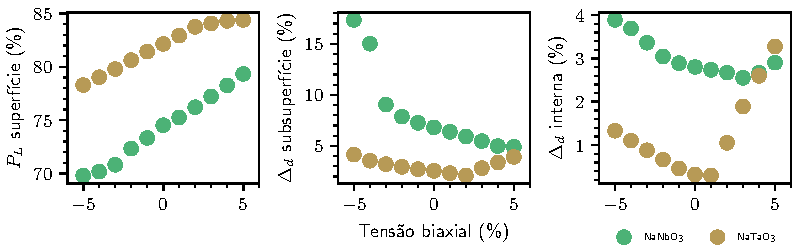
\includegraphics{../floats/geometry_tf_nt_nn/nn_nt_pl_baur_strain_evolution.pdf}
		\caption{Índices de planaridade (superfície) e de deformação (subsuperfície e região interna) dos filmes finos.\label{fig:pl_baur_strain_evolution_NTOvsNNO}}
	\end{figure}
	\begin{equation*}
		\scriptstyle{P_L = \frac{\theta}{\SI{180}{\degree}};\; \Delta_d = \frac{1}{6} \sum^{6}_{i=1} \frac{|d_{\ce{Nb-O}\, i} - \overline{d_{\ce{Nb-O}}}|}{\overline{d_{\ce{Nb-O}}}};}
	\end{equation*}
\end{frame}
\begin{frame}{Evolução Comparada Da Estrutura Eletrônica: Compressão}
	\begin{columns}
		\begin{column}{.5\textwidth}
			\begin{figure}[t]
				\centering
				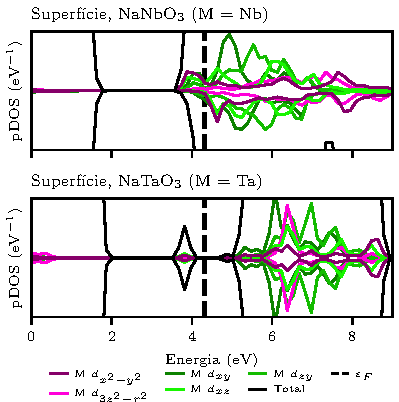
\includegraphics{../floats/pdos_nn_nt_tf/pdos_c5_nn_nt_surface.pdf}
				\caption{DOS projetada da camada superficial do filme fino sob tensão $\epsilon = -5\%$.\label{fig:pdos_c5_nn_nt_surface}}
			\end{figure}
		\end{column}
		\begin{column}{.5\textwidth}
			\begin{itemize}
				\item Em comum: compressão \alert{aumenta} o tamanho de banda proibida;
				\item \ce{NaNbO3}: níveis de superfície hibridizados com a banda de condução, diminui DOS;
				\item \ce{NaTaO3}: níveis de superfície isolados que adentram a banda proibida, diminui DOS;
			\end{itemize}
		\end{column}
	\end{columns}
\end{frame}
\begin{frame}{Evolução Comparada Da Estrutura Eletrônica: Tração}
	\begin{columns}
		\begin{column}{.5\textwidth}
			\begin{figure}[t]
				\centering
				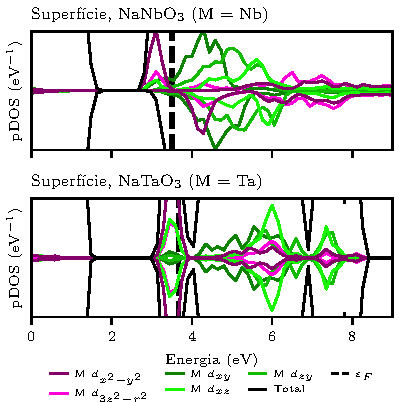
\includegraphics{../floats/pdos_nn_nt_tf/pdos_t5_nn_nt_surface.pdf}
				\caption{DOS projetada da camada superficial do filme fino sob tensão $\epsilon = 5\%$.\label{fig:pdos_t5_nn_nt_surface}}
			\end{figure}
		\end{column}
		\begin{column}{.5\textwidth}
			\begin{itemize}
				\item Em comum: tração \alert{diminui} o tamanho da banda proibida;
				\item \ce{NaNbO3}: níveis de superfície hibridizados com a banda de condução, aumento da DOS;
				\item \ce{NaTaO3}: níveis de superfície isolados que se aproximam da banda de condução, aumento da DOS;
			\end{itemize}			
		\end{column}
	\end{columns}
\end{frame}

%! TEX root = ../root/root.tex 
\section{Conclusões}

\begin{frame}{Recaptulando}
	\begin{block}{Estratégia: Vacâncias Em Cristal Volumoso}
		\begin{itemize}
			\item v$_{\ce{Na}}^0$ insere níveis rasos doadores pois pouco distorce a rede cristalina, formação facilitada por condições oxidantes $\to$ pode potencializar a reação de evolução de oxigênio;
			\item v$_{\ce{O}}^{2+}$ insere níveis rasos próximos à banda de condução, formação facilitada por condições redutoras $\to$ pode reduzir banda proibida $\to$ absorção de luz mais próxima do visível.
		\end{itemize}
	\end{block}
	\begin{block}{Estratégia: Filme Fino}
		\begin{itemize}
		\item Em filme fino nanométrico, orientado em $[100]$, o \ce{NaNbO3} forma estados de superfície metalizados que persistem com tensão biaxial $\to$ necessária outra estratégia para produção de \ce{H2};
		\item Comparação com o \ce{NaTaO3} revela a influência da eletronegatividade: com eletronegatividade menor, \ce{Ta} forma níveis de superfície que podem participar da fotocatálise da água.
		\end{itemize}
	\end{block}
\end{frame}
\begin{frame}{Conclusões e Perspectivas}
	\begin{itemize}
		\item Bandas eletrônicas alinhadas com potenciais de oxirredução da água $+$ absorção de luz visível $+$ condução efetiva de cargas p/ sítios ativos na superfície $=$ fotocatalisador;
		\item Absorção de luz visível aumenta eficiência $+$ níveis eletrônicos das vacâncias podem diminuir a banda proibida $\to$ aumento na eficiência do \ce{NaNbO3} ortorrômbico;
		\begin{itemize}
			\item Melhor descrição dos níveis \ce{Nb} $4d$ $\to$ melhor descrição dos $\Delta E_f$ e níveis de ionização;
		\end{itemize}
		\item Filme fino de \ce{NaNbO3} orientado em $[100]$ e terminado em \ce{NaNbO} não deve ter atividade fotocatalítica $\to$ metalização persiste sob tensão biaxial;
		\item Filme fino de \ce{NaTaO3}, na mesma orientação e terminação, pode ser um fotocatalisador $\to$ níveis de superfície localizados e profundos pela eletronegatividade do \ce{Ta};
		\begin{itemize}
			\item Defeitos de superfície podem fazer os estados de superfície \ce{NaNbO3} se comportarem mais como os de \ce{NaTaO3};
		\end{itemize}
	\end{itemize}
\end{frame}


\begin{frame}
    \vfill
    \centering
    \huge
    \alert{Obrigado!\\Perguntas?}\\\vspace{50px}
    
\includegraphics[height=40px]{../floats/agradecimentos/logo-original-preta.pdf}\quad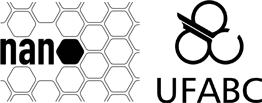
\includegraphics[height=40px]{../floats/agradecimentos/logo_nano_footer2.png}\quad
\includegraphics[height=40px]{../floats/agradecimentos/computacao.png}\\
    
\includegraphics[height=40px]{../floats/agradecimentos/topo_cenapad_unicamp.jpg}
\end{frame}

%! TEX root = ../root/root.tex 
\section*{Anexos}

\begin{frame}[allowframebreaks]{Anexo A -- Informações Suplementares}
    \begin{minipage}{\textwidth}
        \begin{table}[h!]
            \def\arraystretch{1.2}
            \centering
            \caption{Comparação das energias de formação de defeito com carga usando diferentes abordagens para a energia de Fermi ($\varepsilon_F$): a partir do ciclo autoconsistente da DFT, $\varepsilon_F$ no meio da banda proibida e a partir da definição de $\varepsilon_F$ em $T\to0$. Potencial químico veio do equilíbrio E.\label{tab:mudanca-fermi}}
            \resizebox{\textwidth}{!}{%
            \begin{tabular}{lrrrrrr}
            \hline
                                      & \multicolumn{3}{c}{$\Delta E_f (\text{v}_{\ce{O}}^{2+}; L)$ (\si{\electronvolt})}                                                                               & \multicolumn{3}{c}{$\Delta E_f (\text{v}_{\ce{Na}}^{1-}; L)$ (\si{\electronvolt})}                                                                              \\
            $L$                       & \multicolumn{1}{c}{$\varepsilon_F$ da DFT} & \multicolumn{1}{c}{$\varepsilon_F = {}^{E_g}\!/{}_{2}$} & \multicolumn{1}{c}{$\varepsilon_F$ da definição${}^{*}$} & \multicolumn{1}{c}{$\varepsilon_F$ da DFT} & \multicolumn{1}{c}{$\varepsilon_F = {}^{E_g}\!/{}_{2}$} & \multicolumn{1}{c}{$\varepsilon_F$ da definição${}^{*}$} \\\hline
            $1\!\times\!1\!\times\!1$ & $-5,\!72$                                  & $-4,\!27$                                               & $-2,\!41$                                                & $4,\!75$                                   & $4,\!27$                                                & $5,\!03$                                                 \\
            $2\!\times\!2\!\times\!2$ & $-6,\!41$                                  & $-5,\!03$                                               & $-3,\!06$                                                & $5,\!28$                                   & $4,\!62$                                                & $5,\!55$                                                 \\
            $3\!\times\!3\!\times\!3$ & $-5,\!96$                                  & $-4,\!67$                                               & $-2,\!72$                                                & $5,\!62$                                   & $5,\!00$                                                & $5,\!97$                                                 \\
            $L\to\infty$              & $-4,\!60$                                  & $-3,\!53$                                               & $-1,\!66$                                                & $6,\!41$                                   & $5,\!94$                                                & $6,\!98$                                                 \\\hline
            \end{tabular}}
        \end{table}
        \footnotetext{${}^{*}$\cite{shegelski_new_1986}.}
    \end{minipage}\framebreak
    \begin{figure}[h]
        \centering
        \caption{Potencial eletrostático do filme fino de \ce{NaNbO3} orientado em $[100]$, terminado em \ce{NaNbO} e em estado fundamental mostrando o potencial médio na região interna $\tilde{V}_{interna} = \SI{-12.55}{\electronvolt}$ e ``potencial em vácuo'' $V_{vac} = \SI{4.44}{\electronvolt}$.}
        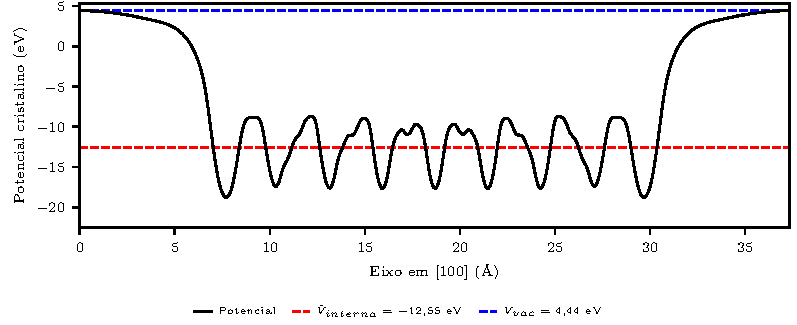
\includegraphics{../floats/vacuum_tf/x_potential.pdf}
    \end{figure}
\end{frame}

\end{document}
